\documentclass[spanish, 11pt, a4paper]{book}
\usepackage[T1]{fontenc} % Use 8-bit encoding that has 256 glyphs
\usepackage[utf8]{inputenc}
\usepackage{fourier} % Use the Adobe Utopia font for the document - comment this line to return to the LaTeX default
\usepackage{listings} % para insertar código con formato similar al editor
%\usepackage{babel} % Selecciona el español para palabras introducidas automáticamente, p.ej. "septiembre" en la fecha y especifica que se use la palabra Tabla en vez de Cuadro [spanish, es-tabla]
\usepackage[spanish,es-tabla]{babel}
\usepackage{url} % ,href} %para incluir URLs e hipervínculos dentro del texto (aunque hay que instalar href)
\usepackage{graphics,graphicx, float} %para incluir imágenes y colocarlas
\usepackage[gen]{eurosym} %para incluir el símbolo del euro
\usepackage{cite} %para incluir citas del archivo <nombre>.bib
\usepackage{enumerate}
\usepackage{hyperref}
\usepackage{graphicx}
\usepackage{tabularx}
\usepackage{booktabs}
\usepackage{array}

\usepackage[table,xcdraw]{xcolor}
\hypersetup{
	colorlinks=true,	% false: boxed links; true: colored links
	linkcolor=black,	% color of internal links
	urlcolor=cyan		% color of external links
}
\renewcommand{\familydefault}{\sfdefault}
\usepackage{fancyhdr} % Custom headers and footers
\pagestyle{fancyplain} % Makes all pages in the document conform to the custom headers and footers
\fancyhead[L]{} % Empty left header
\fancyhead[C]{} % Empty center header
\fancyhead[R]{Luis Aróstegui Ruiz} % My name
\fancyfoot[L]{} % Empty left footer
\fancyfoot[C]{} % Empty center footer
\fancyfoot[R]{\thepage} % Page numbering for right footer
%\renewcommand{\headrulewidth}{0pt} % Remove header underlines
\renewcommand{\footrulewidth}{0pt} % Remove footer underlines
\setlength{\headheight}{13.6pt} % Customize the height of the header

\usepackage{titlesec, blindtext, color}
\definecolor{gray75}{gray}{0.75}
\newcommand{\hsp}{\hspace{20pt}}
\titleformat{\chapter}[hang]{\Huge\bfseries}{\thechapter\hsp\textcolor{gray75}{|}\hsp}{0pt}{\Huge\bfseries}
\titleformat{\part}[hang]{\Huge\bfseries}{\thepart\hsp\textcolor{gray75}{|}\hsp}{0pt}{\Huge\bfseries}
\setcounter{secnumdepth}{4}
\usepackage[Sonny]{fncychap}

% Code Style

%New colors defined below
\definecolor{codegreen}{rgb}{0,0.6,0}
\definecolor{codegray}{rgb}{0.5,0.5,0.5}
\definecolor{codepurple}{rgb}{0.58,0,0.82}
\definecolor{backcolour}{rgb}{0.95,0.95,0.92}

%Code listing style named "mystyle"
\lstdefinestyle{mystyle}{
  backgroundcolor=\color{backcolour}, commentstyle=\color{codegreen},
  keywordstyle=\color{magenta},
  numberstyle=\tiny\color{codegray},
  stringstyle=\color{codepurple},
  basicstyle=\ttfamily\footnotesize,
  breakatwhitespace=false,         
  breaklines=true,                 
  captionpos=b,                    
  keepspaces=true,                 
  numbers=left,                    
  numbersep=5pt,                  
  showspaces=false,                
  showstringspaces=false,
  showtabs=false,                  
  tabsize=2
}

%"mystyle" code listing set
\lstset{style=mystyle}


\begin{document}

	% Plantilla portada UGR
	\begin{titlepage}
 
 
\newlength{\centeroffset}
\setlength{\centeroffset}{-0.5\oddsidemargin}
\addtolength{\centeroffset}{0.5\evensidemargin}
\thispagestyle{empty}

\noindent\hspace*{\centeroffset}\begin{minipage}{\textwidth}

\centering

\includegraphics[width=0.9\textwidth]{imagenes/logo_ugr.jpg}\\[1.4cm]

\textsc{ \Large TRABAJO FIN DE GRADO\\[0.2cm]}
\textsc{ INGENIERÍA EN ...}\\[1cm]
% Upper part of the page
% 
% Title
{\Huge\bfseries Titulo del Proyecto\\
}
\noindent\rule[-1ex]{\textwidth}{3pt}\\[3.5ex]
{\large\bfseries Subtitulo del Proyecto}
\end{minipage}

\vspace{2.5cm}
\noindent\hspace*{\centeroffset}\begin{minipage}{\textwidth}
\centering

\textbf{Autor}\\ {Nombre Apellido1 Apellido2 (alumno)}\\[2.5ex]
\textbf{Directores}\\
{Nombre Apellido1 Apellido2 (tutor1)\\
Nombre Apellido1 Apellido2 (tutor2)}\\[2cm]

\includegraphics[width=0.3\textwidth]{imagenes/etsiit_logo.png}\\[0.1cm]
\textsc{Escuela Técnica Superior de Ingenierías Informática y de Telecomunicación}\\
\textsc{---}\\
Granada, mes de 201
\end{minipage}
%\addtolength{\textwidth}{\centeroffset}
%\vspace{\stretch{2}}
\end{titlepage}



	
	% Plantilla prefacio UGR
	\thispagestyle{empty}

\begin{center}
{\large\bfseries TFG - DASIoT: Desarrollo y Auditoría de Seguridad para prototipo de dispositivos IoT}\\
\end{center}
\begin{center}
Luis Aróstegui Ruiz\\
\end{center}

%\vspace{0.7cm}
\vspace{0.5cm}
\noindent{\textbf{Palabras clave}: Internet de las Cosas, Seguridad}\\

\vspace{0.7cm}
\noindent{\textbf{Resumen}}\\

En el contexto de IoT, hay un ecosistema de entornos de desarrollo específicos. En este TFG se hará uso de alguno de ellos para llevar a cabo la implementación de un dispositivo IoT y analizar los potenciales problemas de seguridad que pueden aparecer durante la etapa de implementación.

% El Internet de las Cosas (IoT) se utiliza para proporcionar conectividad entre diferentes
% dispositivos, los cuales están conectados a Internet. Es un sistema donde los objetos
% actúan con otros objetos a través de un medio de comunicación inalámbrico para
% intercambiar y transferir información sin interacción humana.
% Los dispositivos IoT son propensos a ataques vulnerables debido a la naturaleza simple
% y abierta de sus redes. Por lo tanto, la privacidad y la seguridad son la mayor
% preocupación de esta tecnología. El enfoque de las amenazas de seguridad y privacidad
% en IoT es crucial para promover el desarrollo de IoT.
% Este trabajo final de grado tiene como objetivo conceptualizar el Internet de las Cosas,
% establecer cuáles son sus principales características, y entrar en detalle en los aspectos
% de la privacidad y la seguridad de los datos personales. Cuáles son esas amenazas, la
% problemática particular del Internet de las Cosas que las genera y como mitigar el riesgo
% a dichas amenazas.
% En este trabajo nos haremos las siguientes preguntas: ¿Qué pasa con nuestros datos
% personales? ¿A qué riesgos estamos expuestos aportando tanta información “privada”?
% ¿Qué seguridad existe en el Internet de las Cosas? En este proyecto se pretende
% responder a estas y a muchas otras preguntas. Para ello vamos a profundizar en el tema
% de la privacidad y seguridad en el Internet de las Cosas.

\cleardoublepage


\begin{center}
{\large\bfseries Project Title: Project Subtitle}\\
\end{center}
\begin{center}
First name, Family name (student)\\
\end{center}

%\vspace{0.7cm}
\noindent{\textbf{Keywords}: Keyword1, Keyword2, Keyword3, ....}\\

\vspace{0.7cm}
\noindent{\textbf{Abstract}}\\

Write here the abstract in English.

\cleardoublepage
\thispagestyle{empty}

\noindent\rule[-1ex]{\textwidth}{2pt}\\[4.5ex]

Yo, \textbf{Nombre Apellido1 Apellido2}, alumno de la titulación TITULACIÓN de la \textbf{Escuela Técnica Superior
de Ingenierías Informática y de Telecomunicación de la Universidad de Granada}, con DNI XXXXXXXXX, autorizo la
ubicación de la siguiente copia de mi Trabajo Fin de Grado en la biblioteca del centro para que pueda ser
consultada por las personas que lo deseen.

\vspace{6cm}

\noindent Fdo: Nombre Apellido1 Apellido2

\vspace{2cm}

\begin{flushright}
Granada a X de mes de 201 .
\end{flushright}

\cleardoublepage
\thispagestyle{empty}

\noindent\rule[-1ex]{\textwidth}{2pt}\\[4.5ex]

D. \textbf{Nombre Apellido1 Apellido2 (tutor1)}, Profesor del Área de XXXX del Departamento YYYY de la Universidad de Granada.

\vspace{0.5cm}

D. \textbf{Nombre Apellido1 Apellido2 (tutor2)}, Profesor del Área de XXXX del Departamento YYYY de la Universidad de Granada.


\vspace{0.5cm}

\textbf{Informan:}

\vspace{0.5cm}

Que el presente trabajo, titulado \textit{\textbf{Título del proyecto, Subtítulo del proyecto}},
ha sido realizado bajo su supervisión por \textbf{Nombre Apellido1 Apellido2 (alumno)}, y autorizamos la defensa de dicho trabajo ante el tribunal
que corresponda.

\vspace{0.5cm}

Y para que conste, expiden y firman el presente informe en Granada a X de mes de 201 .

\vspace{1cm}

\textbf{Los directores:}

\vspace{5cm}

\noindent \textbf{Nombre Apellido1 Apellido2 (tutor1) \ \ \ \ \ Nombre Apellido1 Apellido2 (tutor2)}

\chapter*{Agradecimientos}
\thispagestyle{empty}

       \vspace{1cm}


Poner aquí agradecimientos...


	
	% Índice de contenidos
	\newpage
	\tableofcontents

	% Índice de imágenes y tablas
	\newpage
	\listoffigures

	% Si hay suficientes se incluirá dicho índice
	\listoftables 
	\newpage
	

	% Introducción 
	\chapter{Introducción}
	
	% Planificación
	\chapter{Estado del arte}

{\color{blue}

Antes de empezar a desarrollar los objetivos del proyecto es necesario conocer primero los fundamentos del Internet de las Cosas, esto engloba desde su funcionamiento, tipos de arquitecturas hasta los distintos estándares que existen. % Añadir parte de seguridad (normativas)

\section{Internet de las Cosas}

El Internet de las Cosas %(Ngu, Gutierrez, Metsis, Nepal, y Sheng, 2016)
permite que las personas
interactúen con dispositivos de distinto tipo conectados a Internet, como sensores o actuadores. Con
esto, se consigue integrar cualquier objeto del mundo real a Internet, estableciendo relaciones entre
todos ellos y cambiando la forma en la que interaccionamos con nuestro entorno. \\

La premisa básica y el objetivo de IoT es "conectar lo que no está conectado". Esto significa que los objetos que no están actualmente unidos a una red informática, es decir, a Internet, se conectarán para que puedan comunicarse e interactuar con personas y otros objetos. IoT es una transición tecnológica en la que los dispositivos nos permitirán sentir y controlar el mundo físico haciendo que los objetos sean más inteligentes y conectándolos a través de una red inteligente. 1 Cuando los objetos y las máquinas pueden ser detectados y controlados a distancia a través de una red, se consigue una mayor integración entre el mundo físico y los ordenadores. Esto permite mejoras en las áreas de eficiencia, precisión, automatización y habilitación de aplicaciones avanzadas. \\

El mundo del IoT es amplio y puede resultar algo complicado al principio debido a la abundancia de componentes y protocolos que engloba. En lugar de considerar IoT como un único tecnología, es bueno verlo como un paraguas de varios conceptos, protocolos y tecnologías, todos ellos dependientes a veces de un sector concreto. Aunque la amplia gama de elementos de IoT está diseñado para crear numerosos beneficios en las áreas de productividad y automatización, al mismo al mismo tiempo, introduce nuevos retos, como la ampliación del gran número de dispositivos y de la cantidad de datos que deben procesarse. que hay que procesar. \cite{hanes2017iot}

}

	% Planificación
	\part{Propuesta}

\chapter{Planificación}

\section{Planificación a priori}

Se trata de planificar como se espera desarrollar el proyecto en el tiempo, para ello se va a hacer uso de un diagrama de Gantt donde se va a proporcionar una vista general de las tareas programadas, estas tareas tendrán que completarse en unas fechas estipuladas.

\subsection{Diagrama de Gantt}

Un diagrama de Gantt es una herramienta útil para planificar proyectos. Proporciona una vista general de las tareas programadas, indicando el periodo de tiempo que tienen para completarse.\\

El diagrama se mostrará:
\begin{itemize}
    \item Fecha de inicio y finalización del proyecto.
    \item Las tareas del proyecto.
    \item Fecha de programada de cada tarea, tanto la de inicio como la de final.
    \item Como se superponen las tareas y si hay relación entre ellas.
\end{itemize}

Con esta planificación se conseguirá una mayor claridad en las tareas a realizar y una mejor gestión del tiempo.

\subsection{Etapas de desarrollo}

\begin{itemize}
    \item \textbf{1ª etapa}: Revisar frameworks para IoT.
    \item \textbf{2ª etapa}: Desarrollar aplicación para IoT.
    \item \textbf{3ª etapa}: Explotación de una vulnerabilidad.
    \item \textbf{4ª etapa}: Documentación.
\end{itemize}

\subsection{Temporización}

De los 3 meses y medios a que se van a dedicar al proyecto, en todos ellos se va a desarrollar las etapas indicadas anteriormente. Se muestra la fecha de inicio y de fin de cada etapa.

\renewcommand{\arraystretch}{1.5}\label{presupuesto-section}
\begin{table}[H]
	\centering
	\label{tabla-temporal}
	\resizebox{\textwidth}{!}{%
	\begin{tabular}{@{}ccc@{}}
		\toprule
		\rowcolor[HTML]{ECF4FF} 
		\textbf{Etapas del desarrollo}                                                                                                                  & \textbf{Fecha de comienzo} & \textbf{Fecha de finalización} \\ \midrule
		\cellcolor[HTML]{ECF4FF}\textbf{\begin{tabular}[c]{@{}c@{}}Documentación del proyecto\end{tabular}} & 9 de Marzo                & 23 de Junio                     \\
		\rowcolor[HTML]{EFEFEF} 
		\cellcolor[HTML]{ECF4FF}\textbf{Revisar frameworks IoT}                                                                                & 21 de Marzo                 & 6 de Abril                    \\
		\cellcolor[HTML]{ECF4FF}\textbf{\begin{tabular}[c]{@{}c@{}}Desarrollar aplicación para IoT\end{tabular}}         & 7 de Abril                & 12 de Mayo                    \\
		\rowcolor[HTML]{EFEFEF} 
		\cellcolor[HTML]{ECF4FF}\textbf{Explotar vulnerabilidad}                                                                                   & 13 de Mayo                & 22 de Junio                     \\ \bottomrule
	\end{tabular}}
	\caption{Organización temporal del proyecto.}
\end{table}

\begin{figure}[ht!]
    \centering
    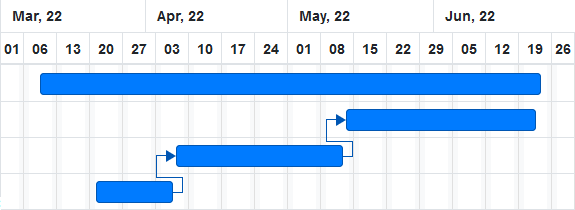
\includegraphics[width=\linewidth]{imagenes/diagramaGantt_v2.png}
    \caption{Diagrama de Gantt. Gráfico.}
    \label{fig:figure3}
\end{figure}

Este gráfico corresponde con la duración de cada etapa, comenzando con la documentación. También se indica que hay etapas que para que estas se puedan empezar a desarrollar necesitan que la anterior este terminada, es el caso de la etapa de \textit{Desarrollo de la aplicación} y de \textit{Explotación de una vulnerabilidad}.

\subsection{Seguimiento del desarrollo}

Con el fin de facilitar la visualización del progreso del proyecto se usan distintas herramientas.

\subsubsection{Trello}

Permite gestionar proyectos de forma sencilla y muy visual. Por cada proyecto se crea un tablero donde podemos crear listas y cada lista almacenará \textit{tarjetas} donde se describirá una tarea u objetivo a cumplir. En nuestro caso el tablero se divide en 7 listas:

\begin{itemize}
    \item \textbf{Dudas}, se dejan ancladas preguntas a los tutores.
    \item \textbf{Objetivos}, para recordar los objetivos que se tienen que completar para el proyecto.
    \item \textbf{Pendientes}, tareas que se tienen que realizar pero no se están desarrollando.
    \item \textbf{En proceso}, tareas que se están trabajando.
    \item \textbf{Pendientes de revisión}, tareas finalizadas que requieren de revisión por parte de los tutores.
    \item \textbf{Terminadas}, tareas que han sido aceptadas en la revisión.
    \item \textbf{Hitos}, se agrupan tareas que forman parte de una misma etapa.
\end{itemize}

\subsubsection{Github}

Se ha creado un repositorio \footnote{Enlace al repositorio: https://github.com/LuisArostegui/TFG} donde se van añadiendo \textit{issues} por cada tarea que se tenga que realizar. Esta tarea es la misma que nos encontramos en el tablero de Trello, por tanto, cuando se crea una nueva tarea en Trello, creamos un nuevo issue con el mismo nombre y descripción para seguir un progreso coherente.\\

También se crean \textit{Milestones} que se corresponde con el nombre y descripción de la lista de \textit{Hitos} del tablero de Trello.\\

Cada vez que terminemos de trabajar en un \textit{Milestone} se creará un \textit{Pull Request} para que los tutores puedan revisar los cambios del proyecto y aceptarlos o rechazarlos. Cada acción que se realice tanto en Trello como en Github se verá reflejado en ambos, de esta manera conseguimos un desarrollo del proyecto realista de principio a final.

\subsubsection{Clockify}

Esta herramienta nos permite seguir el tiempo que estamos trabajando. Cada vez que nos pongamos a trabajar, iniciaremos el contador y nombraremos a ese contador con el nombre de la tarea que estemos realizando en ese momento.

\section{Planificación a posteriori}

Una vez terminado el proyecto nos apoyamos en las distintas herramientas que usamos en la planificación a priori para ver el resultado final. \\

Usando la herramienta de ``Insights`` de Github obtenemos los siguientes resultados:


\begin{figure}[hb!]
    \centering
    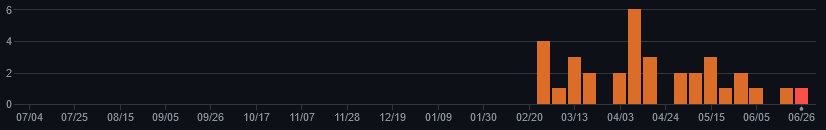
\includegraphics[width=\linewidth]{imagenes/commits.png}
    \caption{Commits realizados por fecha}
    \label{fig:figure4-plan}
\end{figure}

\begin{figure}[hb!]
    \centering
    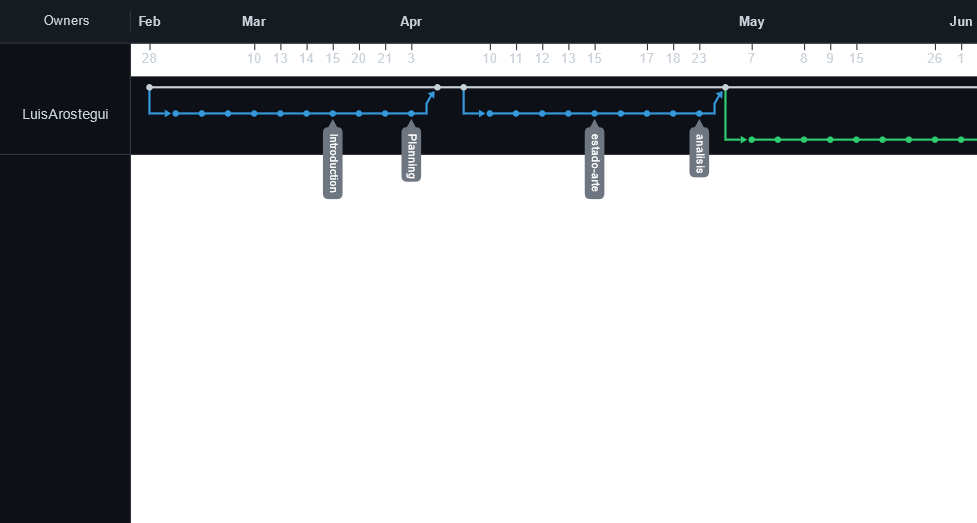
\includegraphics[width=\linewidth]{imagenes/canvas.png}
    \caption{Ramas creadas y forks. Primera parte}
    \label{fig:figure5-plan}
\end{figure}

\begin{figure}[ht!]
    \centering
    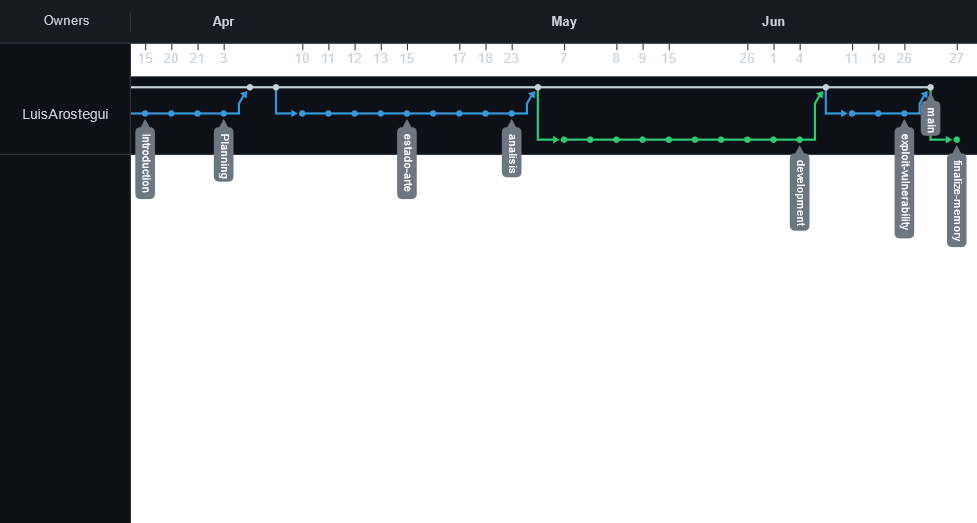
\includegraphics[width=\linewidth]{imagenes/canvas2.png}
    \caption{Ramas creadas y forks. Segunda parte}
    \label{fig:figure6-plan}
\end{figure}

Se empezó a trabajar en Marzo, tal y como se indicó en la planificación pero la finalización del primer objetivo se retrasó hasta el 24 de Abril, pero esto se debe a que se realizó un estudio del paradigma IoT y se fue implementando antes la introducción y sección de estado del arte para hacer un trabajo más completo en el primer objetivo. El desarrollo terminó el 5 de Junio y la explotación de la vulnerabilidad y toda su documentación correspondiente el 26 de Junio. En total se ha retrasado 4 días más de lo previsto. \\

\newpage

Por parte de Trello, nos encontramos que conforme se iba avanzando con el proyecto se han creado tarjetas que se correspondían con Milestones o con issues, el resultado es el siguiente:

\begin{figure}[hb!]
    \centering
    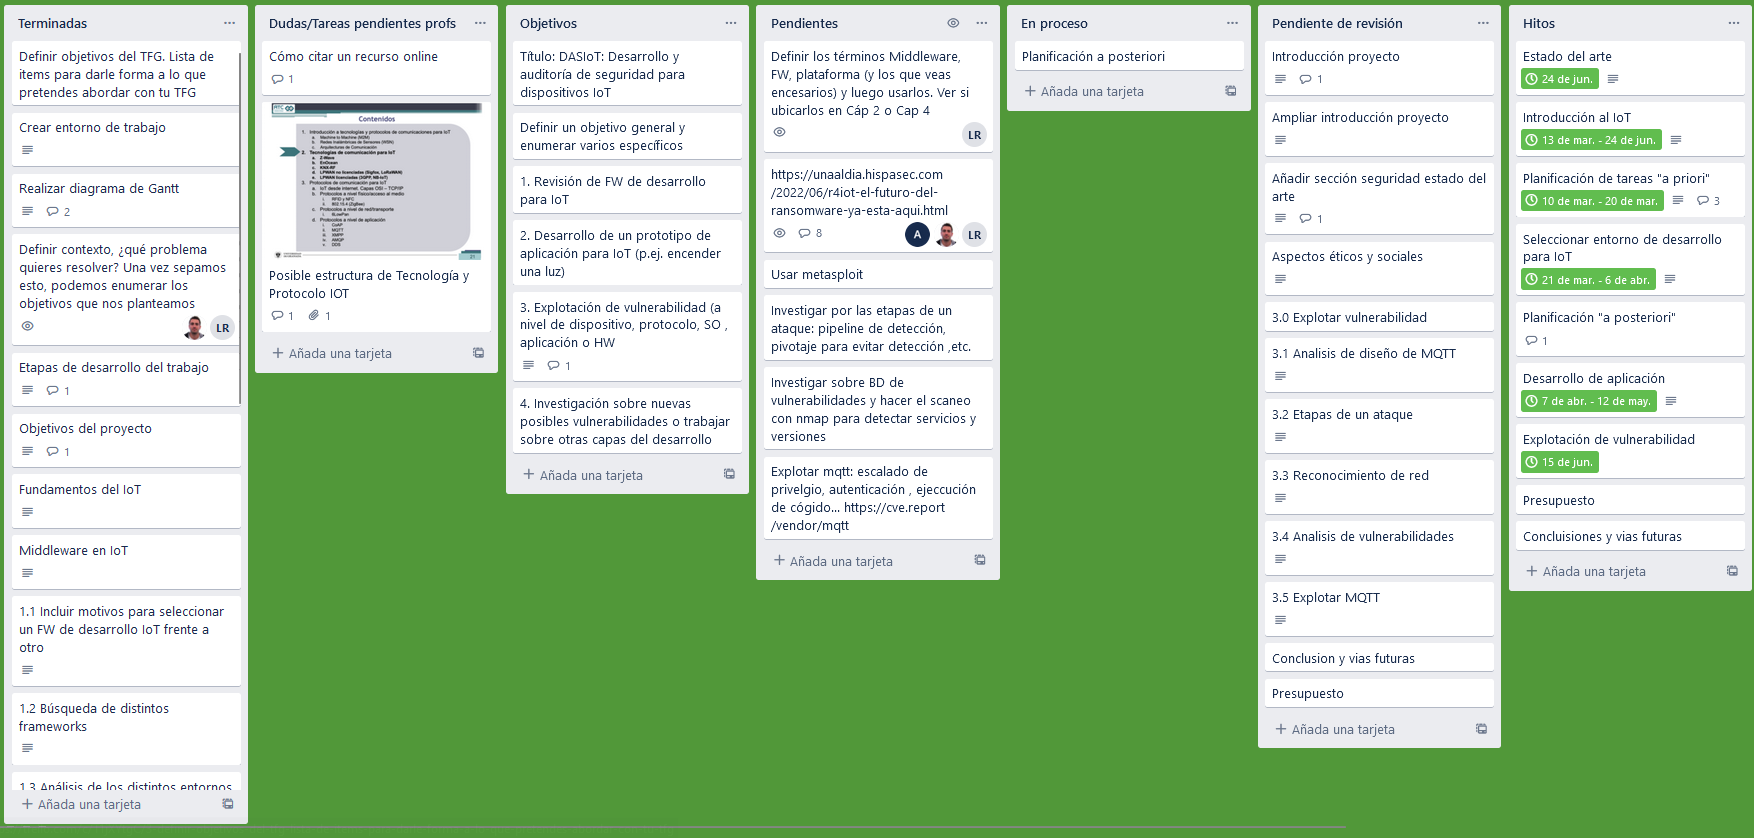
\includegraphics[width=\linewidth]{imagenes/trello.png}
    \caption{Tarjetas creadas en el proyecto en Trello}
    \label{fig:figure7-plan}
\end{figure}

\newpage

Y en clockify este es el seguimiento del tiempo dedicado a cada tarea (correspondiente a la tarjeta de Trello):


\begin{figure}[hb!]
    \centering
    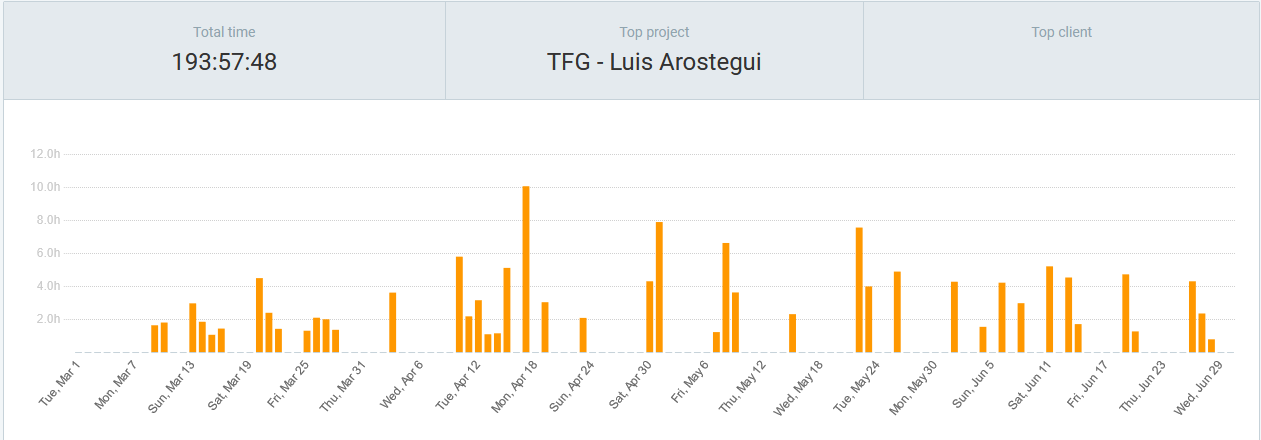
\includegraphics[width=\linewidth]{imagenes/clockify.png}
    \caption{Tiempo dedicado. Clockify.}
    \label{fig:figure8-plan}
\end{figure}




\chapter{Presupuesto}

En una situación donde estemos contratados por una entidad que requiera de nuestros servicios para la auditoría de seguridad de dispositivos IoT, que requiera de la investigación y análisis del paradigma IoT. Teniendo en cuenta que al ser un ingeniero informático sin experiencia laboral, trabajando 5 horas al día, durante 5 días a la semana, un total de 300 horas en 3 meses. Para calcular el precio de la mano de obra, se tiene en cuenta lo que suele cobrar un ingeniero informático sin experiencia, unos 22 mil euros al año a jornada completa, esto se ve reflejado en 6.12€ a la hora, lo que hace un total de 1836€. \\

Se debe de tener en cuenta las ayudas que se obtienen por parte de la universidad, en este caso se trata de toda la bibliografía a la que podemos acceder. Si no pudiésemos acceder gratuitamente a estos libros, teniendo en cuenta la bibliografía usada obtenemos un gasto de \textbf{950€}. Se ha usado la web de \textit{Amazon.es} para buscar los precios de todos los libros, a día 7 de Julio de 2022.

Una vez vista la mano de obra, se ve el coste de los materiales.

\renewcommand{\arraystretch}{1.5}\label{time-section}
\begin{table}[H]
	\centering
	\label{tabla-presupuesto}
	\resizebox{\textwidth}{!}{%
	\begin{tabular}{@{}ccc@{}}
		\toprule
		\rowcolor[HTML]{ECF4FF} 
		\textbf{Descripción}                                                                                                                  & \textbf{Importe por unidad} & \textbf{Total} \\ \midrule
		\cellcolor[HTML]{ECF4FF}\textbf{\begin{tabular}[c]{@{}c@{}}Mano de obra\end{tabular}} & 1836€                & 1836€                     \\
		\rowcolor[HTML]{EFEFEF} 
		\cellcolor[HTML]{ECF4FF}\textbf{Ordenador de sobremesa para desarrollo}                                                                                & 1600€                 & 1600€                    \\
				\rowcolor[HTML]{EFEFEF} 
		\cellcolor[HTML]{ECF4FF}\textbf{Libros}                                                                                & 950€                 & 950€                    \\
		\rowcolor[HTML]{EFEFEF} 
		\cellcolor[HTML]{ECF4FF}\textbf{Raspberry PI}                                                                                & 40€                 & 40€                    \\
		\cellcolor[HTML]{ECF4FF}\textbf{\begin{tabular}[c]{@{}c@{}}SanDisk Extreme Tarjeta de Memoria microSD de 64 GB\end{tabular}}         & 20€                & 20€                    \\
		\rowcolor[HTML]{EFEFEF} 
		\cellcolor[HTML]{ECF4FF}\textbf{Instalación y mantenimiento de los componentes y software}                                                                                   & 100€                & 100€                     \\
		\cellcolor[HTML]{ECF4FF}\textbf{\textbf{Total completo}}                                                                                   & \textbf{4546€}               &                      \\\bottomrule
	\end{tabular}}
	\caption{Presupuesto total del proyecto.}
\end{table}



\chapter{Análisis del problema}
{\color{blue}

Siguiendo los objetivos del proyecto \ref{sec:objetivos} se va a analizar los diferentes frameworks que existen para desarrollar una aplicación para posteriormente analizar posibles explotaciones de seguridad. \\

Como hemos visto en \ref{sec:iot}, normalmente, cuando se generan grandes datos y se transmiten a través de varios dispositivos, tiene que haber un punto específico en el que se recoja y combine todo. Este punto específico es muy esencial en una red, ya que combina todos los datos, lo que permite comprender los datos que se generan. Sin embargo, la transmisión y generación de datos sin problemas no se produce sin más. Más bien, suele ser posible gracias a un framework del Internet de las Cosas. \\

Un framework para IoT puede describirse como un ecosistema, compuesto por varios dispositivos conectados que se comunican entre sí, a través de Internet. Estos dispositivos conectados suelen funcionar para transferir y detectar datos a través de Internet, y requieren muy poca intervención humana. El framework de IoT es lo que hace posible que los dispositivos conectados tengan una comunicación fluida a través de Internet. Es un elemento tecnológico muy importante en el mundo moderno, que encuentra aplicación en casi todos los sectores. Por ejemplo, una de las principales aplicaciones del IoT es el diseño de casas inteligentes. \cite{iot-framework}\\

Es decir, un framework para IoT recoge todos principales elementos que componen el mundo del Internet de las Cosas para desarrollar una aplicación, estos elementos los podemos ver en la siguiente imagen \ref{fig:figure4}.

\begin{figure}[ht!]
    \centering
    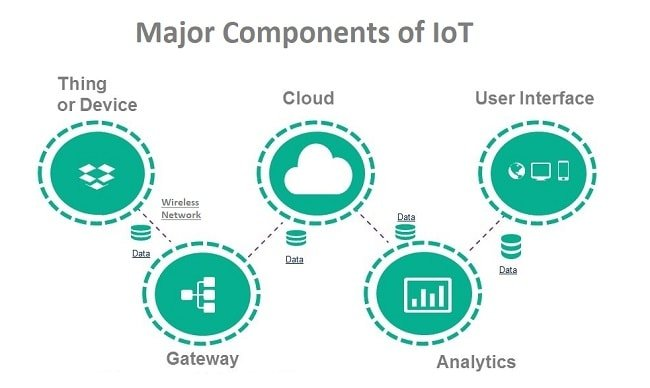
\includegraphics[width=\linewidth]{imagenes/Key-IoT-Components.jpg}
    \caption{Elementos principales de un framework en IoT. \cite{key-iot-framework}}
    \label{fig:figure4}
\end{figure}

\newpage

Cuando se esta desarrollando una aplicación, el concepto de ``framework`` se puede relacionar con otros conceptos como el de ``middleware`` y ``plataforma``. El concepto de ``plataforma`` hace referencia al lugar donde se permite desplegar y ejecutar la aplicación. Por otro lado el middleware, tiene que ver con la prestación de los servicios. Y por último, el framework se centra más en el diseño del software. Por esto, pese a que en este proyecto se va a trabajar con un framework, hay que tener en cuenta otros conceptos que rodean al desarrollo de una aplicación. \cite{nakhuva2015study}

\section{Middleware} \label{sec:middleware}

Generalmente, un middleware abstrae las complejidades del sistema o del hardware, permitiendo al desarrollador de la aplicación centrar todo su esfuerzo en la tarea a resolver, sin la distracción de preocupaciones a nivel del sistema o del hardware. Dichas complejidades pueden estar relacionadas con problemas de comunicación o de computación más generales. Un middleware proporciona una capa de software entre las aplicaciones, el sistema operativo y las capas de comunicación de la red, que facilita y coordina que facilita y coordina algún aspecto del procesamiento cooperativo. Desde el punto de vista perspectiva informática, un middleware proporciona una capa entre el software de aplicación y el software de sistema.\\

En el IoT, es probable que haya una considerable heterogeneidad tanto en las tecnologías de comunicación en uso, como en las tecnologías a nivel de sistema, y un middleware debe soportar ambas perspectivas según sea necesario. 

Basándonos en las características descritas anteriormente \ref{sec:iot} de la infraestructura del IoT y de las aplicaciones que dependen de ella, se establecen un conjunto de requisitos para que un middleware soporte el IoT. A continuación, estos requisitos se agrupan en dos conjuntos: los servicios que debe proporcionar dicho middleware y la arquitectura del sistema \cite{7322178}-\cite{7582463}.

\subsection{Requisitos del servicio de middleware}

 Los requisitos de los servicios de middleware para el IoT pueden clasificarse en funcionales y no funcionales. Los requisitos funcionales recogen los servicios o funciones, como por ejemplo abstracciones y gestión de recursos un middleware, y los requisitos no funcionales, por ejemplo fiabilidad, seguridad y disponibilidad, captan el soporte de la calidad de servicio o del rendimiento.\\
 
 En los requisitos funcionales nos encontramos:
 
 \begin{itemize}
     \item \textbf{Descubrimiento de recursos}. Ya que la infraestructura y el entorno del IoT son dinámicos, las suposiciones relacionadas con el conocimiento global y determinista de la disponibilidad de estos recursos es inviable. Pasa lo mismo con la intervención humana, es inviable que este descubra recursos. Por tanto, es importante destacar que el descubrimiento de recursos este automatizado. Cuando no hay infraestructura, el propio dispositivo debe de anunciar su presencia y los recursos que ofrece.
     \item \textbf{Gestión de recursos}. Se espera una QoS (Quality of Service) aceptable para todas las aplicaciones, y en un entorno en el que los recursos que influyen en la QoS son limitados, como el IoT, es importante que las aplicaciones cuenten con un servicio que gestione esos recursos.
     \item \textbf{Gestión de datos}. Los datos son fundamentales en las aplicaciones de IoT. En el IoT, los datos se refieren principalmente a los datos detectados o a cualquier información de infraestructura de red de interés para las aplicaciones.
     \item \textbf{Gestión de eventos}. En las aplicaciones de IoT se genera potencialmente un número masivo de eventos, que deberían gestionarse como parte integral de un middleware de IoT.
     \item \textbf{Gestión del código}. El despliegue de código en un entorno de IoT es un reto, y debe ser soportado directamente por el middleware. En particular, se necesitan servicios de asignación y de código.
 \end{itemize}
 
 En los requisitos no funcionales nos encontramos:
 
  \begin{itemize}
     \item \textbf{Escalabilidad}. Un middleware de IoT debe ser escalable para adaptarse al crecimiento de la red y las aplicaciones/servicios de IoT.
     \item \textbf{Actuación en tiempo real}. Un middleware debe proporcionar servicios en tiempo real cuando la corrección de una operación que soporta depende no sólo de su corrección lógica sino sino también del tiempo en que se realiza.
     \item \textbf{Fiabilidad}. Un middleware debe permanecer operativo durante la duración de una misión, incluso en presencia de fallos.
     \item \textbf{Disponibilidad}. Un middleware que soporte las aplicaciones de un IoT, especialmente las de misión crítica, debe estar disponible en todo momento.
     \item \textbf{Seguridad y privacidad}. La seguridad es fundamental para el funcionamiento de IoT. En el middleware de IoT, la seguridad debe tenerse en cuenta en todos los bloques funcionales y no funcionales, incluyendo la aplicación a nivel de usuario.
     \item \textbf{Facilidad de despliegue}. Hay que evitar los procedimientos complicados de instalación y configuración.
     \item \textbf{Popularidad}. Un middleware de IoT, como cualquier otra solución de software, debe recibir un apoyo y una ampliación continua.
 \end{itemize}
 
\subsection{Requisitos de arquitectura en el middleware}

En esta sección se muestran los requisitos para las abstracciones de programación y otros aspectos relacionados con la implementación.

\begin{itemize}
    \item \textbf{Abstracción de la programación}. Para el desarrollador de aplicaciones o servicios, las interfaces de programación de alto nivel deben aislar el desarrollo de las aplicaciones o los servicios de las operaciones proporcionadas por las infraestructuras subyacentes y heterogéneas del IoT. 
    \item \textbf{Interoperabilidad}. Un middleware debe funcionar con dispositivos, tecnologías y aplicaciones heterogéneas, sin esfuerzo adicional por parte del desarrollador de aplicaciones o servicios.
    \item \textbf{Basado en el servicio}. Una arquitectura de middleware debe estar basada en servicios para ofrecer una gran flexibilidad cuando sea necesario añadir funciones nuevas y avanzadas al middleware de un IoT.
    \item \textbf{Adaptable}. Un middleware debe ser adaptativo para poder evolucionar y adaptarse a los cambios de su entorno.
    \item \textbf{Consciente del contexto}. El conocimiento del contexto es un requisito clave en la construcción de sistemas adaptativos y también en el establecimiento de valor de los datos recogidos.
    \item \textbf{Autónomo}. Los dispositivos, tecnologías y aplicaciones son participantes activos en los procesos del IoT y deben estar habilitados para interactuar y comunicarse entre sí sin la intervención intervención humana.
    \item \textbf{Distribuido}.  Las aplicaciones de un sistema IoT a gran escala de un sistema IoT intercambian información y colaboran entre sí.
\end{itemize}


\section{Frameworks IoT}

Una vez hemos visto requisitos que necesitamos en nuestro middleware, se van a comentar una serie de requisitos que buscamos en nuestro framework IoT. \cite{agarwal2020investigating}-\cite{dumitru2017iot}-\cite{nakhuva2015study}

\subsection{Requisitos para seleccionar un framework IoT} \label{requisitosFramework}

Algunos requisitos principales en los que nos tenemos que fijar a la hora de seleccionar un entorno de desarrollo son:

\begin{itemize}
    \item \textbf{Seguridad y privacidad}. El framework debe de proporcionar seguridad en la capa de transporte para conexiones seguras (encriptación SSL) y no comprometer en el entorno de trabajo. Con esto, conseguimos privacidad, autenticación e integridad en los datos. 
    \item \textbf{Dificultad de uso}. Seleccionar un framework que sea sencillo de usar para desarrolladores. Esto incluye el lenguaje de programación que se use para hacer la aplicación.
    \item \textbf{Código abierto}. Se trata de evitar aquellos framework en los que hay que pagar por su uso o que den un periodo de prueba gratuito. Las plataformas de código abierto permiten que las plataformas sean gestionadas por el desarrollador según sus necesidades.
    \item \textbf{Soporte}. Se busca un framework que sea popular y tenga un equipo y comunidad activa, que continuamente este aportando nuevas características al proyecto.
\end{itemize}

También existen otras características en las que nos podemos fijar que pueden resultar útiles dependiendo del tipo de aplicación que queremos desarrollar:

\begin{itemize}
    \item \textbf{Tipo de soporte de protocolo de comunicación}. Los dispositivos IoT soportan múltiples protocolos de comunicación. Algunos son ligeros y otros son seguros. El protocolo a elegir depende de los requisitos de la aplicación IoT. CoAP es similar a HTTP pero es ligero, por lo que es más adecuado para aplicaciones móviles. MQTT también es ligero y soporta el concepto de broker, por lo que es bueno para aplicaciones de ancho de banda limitado. CoAP es bueno para la multidifusión y la difusión.
    \item \textbf{Disponibilidad}. La disponibilidad y la estabilidad son parámetros importantes para los requisitos del IoT. Por ejemplo, una aplicación enfocada a la salud requiere que los datos datos médicos del paciente para ser monitorizados continuamente.
    \item \textbf{Tecnologías de almacenamiento utilizadas}. Diferentes tecnologías de almacenamiento y procesamiento sobre la nube soportan diferentes tipos de análisis. Según los requisitos de procesamiento de datos, se puede seleccionar una nube con diferentes tecnologías de almacenamiento.
    \item \textbf{Tipo de análisis soportado}. Las aplicaciones de IoT suelen requerir datos en tiempo real o datos históricos para el desarrollo de la aplicación. La elección de la tecnología adecuada para aplicar la analítica al tipo de datos generados por el dispositivo en la aplicación es otro factor importante.
\end{itemize}

\subsection{Varios framework IoT}

\subsubsection{KAA IoT}
    Es totalmente gratis, tiene capacidad para gestionar millones de sensores, recoger y analizar datos en tiempo real y visualizarlos, gestionar y conectar productos inteligentes con ayuda de nube. Permite la gestión de los datos de los objetos conectados y la infraestructura de back-end que proporciona los componentes del SDK del servidor y del endpoint. KAA proporciona la funcionalidad de back-end necesaria para operar una solución IoT. Proporciona flexibilidad a los usuarios para implementar sus propias políticas de seguridad.\\ 
    
    Kaa proporciona un gateway que aporta la posibilidad de conectar diferentes redes entre si. Los protocolos de comunicación que usa para comunicarse con los dispositivos son MQTT y COAP. Para especificar un dispositivo se hace en JSON, donde cada dispositivo es un objeto. Kaa permite el análisis de datos y para ello usa tecnologías como NoSQL, Cassandra, Hadoop y MongoDB. Kaa soporta lenguajes de programación como Java, C, C++. \cite{kaaiot}
    
\subsubsection{ThingSpeak}

Es un framework que se caracteriza por sus visualizaciones y predicciones utilizando MATLAB. Soporta datos con formato JSON y XML. Es de código abierto. Soporta múltiples dispositivos y permite utilizar protocolos como MQTT o Rest API para la comunicación entre dispositivos. Proporciona seguridad en la capa de transporta con encriptación en las comunicaciones. \cite{thingspeak}

\subsubsection{Macchina.io}

Este framework se divide en dos productos, el primero es el \textbf{Edge} que permite que las aplicaciones se ejecuten en dispositivos basados en Linux utilizando C++ y Javascript. Y el segundo producto es el \textbf{Remote} que permite gestionar la infraestructura mediante paneles web y aplicaciones móviles. Una de las tecnologías que utiliza es SQLite e incluye soporte para protocolos de comunicación como MQTT, SOAP, HTTP. \cite{macchinaio}
 
\subsubsection{Altair (Carriots)}

Altair, anteriormente ``Carriots``, es una plataforma diseñada para proyectos IoT. Permite integrar los dispositivos de IoT a una aplicación externa que requiera de los datos mientras ellos se encargan del almacenamiento y la comunicación. Soporta XML, JSON y API Rest. No es gratis, tiene un plan de subscripción. Permite escribir aplicaciones en Java. Para la comunicación entre dispositivos usa MQTT, no posee encriptación en la comunicación pero si posee un mecanismo de autenticación y autorización. Para el almacenamiento usa NoSQL. \cite{altair}

\subsubsection{Zetta}

Es una plataforma de código abierto construida sobre Node.js para crear servidores del Internet de las Cosas que se ejecutan a través de ordenadores geodistribuidos y la nube. Zetta combina las API de REST, los WebSockets y la programación reactiva, lo que resulta perfecto para ensamblar muchos dispositivos en aplicaciones de uso intensivo de datos en tiempo real. Zetta tiene la capacidad de convertir cualquier dispositivo en una API. Al comunicarse con microcontroladores como Arduino y Spark Core, Zetta puede proporcionar a cada dispositivo una API REST tanto localmente como en la nube. Zetta es ``developer friendly`` lo que significa que es sencillo desarrollar usando esta plataforma. Entre las tecnologías que usa esta API Rest y JSON. \cite{zetta}

\subsubsection{Temboo}

Es un framework que entra dentro de la categoría de plataformas que son ``developer friendly``, es decir, para conectar dispositivos y hacer tareas simples se hace de manera rápida y sin complicaciones en el código. Soporta datos en Excel, CSV, XML y JSON. Soporta lenguajes de programación como C, Java, Python y Javascript. No es gratuito, requiere de un plan de subscripción para empezar a utilizarlo. Tiene soporte con múltiples dispositivos, entre ellos Arduino y a destacar Samsung Artik. Los protocolos que soporta son HTTP, MQTT, CoAP. Y tiene soporte de tecnologías como Microsoft Power BI y Google BigQuery. \cite{temboo}

\subsubsection{Particle}

Particle es una plataforma de IoT escalable, fiable y segura. Una característica clave es la capacidad de ejecutar código de cableado de Arduino y Raspberry Pi haciendo más fácil conectar componentes electrónicos a la nube. Los primeros 100 dispositivos que se conecten son gratuitos. En cuanto a la seguridad, es uno de los frameworks con más características relacionadas con esta, posee encriptación en las comunicaciones, autenticación, autorización y posibilidad de auditoría de seguridad, todo esto bajo el protocolo HTTP. Soporta datos en formato CSV y se puede desarrollar código Javascript y en particle js, una librería ligera de Javascript.

\subsubsection{Soluciones comerciales}

Hay otras soluciones comerciales donde nos encotramos plataformas como AWS IoT, Microsoft Azure IoT Hub, IBM Watson IoT, Google IoT y Oracle IoT. Todas estas alternativas son bastante similares a todas las comentadas hasta el momento, se diferencian entre si por ciertas características como el soporte en lenguajes de programación, donde aparecen lenguajes que no vemos en otras plataformas como son Ruby, .NET, Go, php. En la siguiente tabla se muestran características de estas plataformas : 


\begin{table}[H]
	\centering
	\label{tabla-commercial-solutions}
	\resizebox{\textwidth}{!}{%
	\begin{tabular}{ | m{3.5cm} | m{2cm} | m{3cm} | m{2cm} | m{3cm} |}
		\toprule
		\rowcolor[HTML]{ECF4FF} 
		\textbf{Framework IoT} & \textbf{Soporte de datos} & \textbf{Soporte de lenguajes de programación} & \textbf{Protocolos} & \textbf{Seguridad} \\ \midrule
		\cellcolor[HTML]{ECF4FF}\textbf{\begin{tabular}[c]{@{}c@{}}AWS IoT\end{tabular}} & JSON                & Java, C, NodeJS, Javascript, Python, iOS, Android & HTTP, MQTT, Websockets & Encriptación, autenticación, autorización, auditoría                  \\
		\cellcolor[HTML]{ECF4FF}\textbf{\begin{tabular}[c]{@{}c@{}}Microsoft Azure IoT\end{tabular}} & JSON  & .NET, UWP, Java, C, NodeJS, Ruby, Android, iOS & HTTP, AMQP & Encriptación, autenticación, autorización, políticas definidas por usuario                   \\
		\cellcolor[HTML]{ECF4FF}\textbf{\begin{tabular}[c]{@{}c@{}}IBM Watson IoT\end{tabular}} & JSON, CSV  & C\#, C, Python, Java, NodeJS & MQTT & Autenticación, Autorización                  \\
		\cellcolor[HTML]{ECF4FF}\textbf{\begin{tabular}[c]{@{}c@{}}Oracle IoT\end{tabular}} & JSON, CSV  & Java, Javascript, Android, C, iOS & REST API & Autenticación, Autorización \\
		\cellcolor[HTML]{ECF4FF}\textbf{\begin{tabular}[c]{@{}c@{}}Google IoT\end{tabular}} & JSON                & Go,Java, .NET, Node.js, php, Python, Ruby & MQTT, HTTP & Autenticación                  \\ \bottomrule
	\end{tabular}}
	\caption{Características de soluciones comerciales para framework IoT. \cite{agarwal2020investigating}}
\end{table}

\section{Elección del framework} \label{eleccion-framework}

Como framework para desarrollar la aplicación se ha optado por trabajar con \textbf{Kaa IoT}. La motivación de su uso viene de cumplir todos los requisitos establecidos en la sección \ref{requisitosFramework}.

\begin{itemize}
    \item \textbf{Seguridad y privacidad}. Kaa IoT proporciona autenticación del cliente con certificado SSL/TLS, por tanto, todas sus comunicaciones van a estar cifradas. Aparte, para el proyecto puede resultar útil posible implementación de nuestras propias políticas de seguridad.
    \item \textbf{Dificultad de uso}. No llega a ser un framework ``developer friendly``, pero en la documentación del framework \cite{kaaiot} hay varios tutoriales como para desarrollar sin mucha dificultad una aplicación , explicando en cada apartado las palabras clave o conceptos que se necesitan para entender todo lo que se esta haciendo en la construcción de la aplicación. Aquellos frameworks ``developer friendly``, por el hecho de ser plataformas donde ofrecen ayudar por desarrollar y desplegar la aplicación requieren de una subscripción para hacer uso de estas.
    \item \textbf{Código abierto}. Es un framework gratuito, evitamos todos los frameworks que requieren de un plan de subscripción.
    \item \textbf{Soporte}. Es de los frameworks más conocidos. Y tienen una comunidad activa, esto se puede observar en su repositorio de github \footnote{Enlace a repositorio de Kaa IoT: https://github.com/kaaproject/kaa}, que cada poco tiempo van añadiendo nuevas características y documentación al proyecto.
\end{itemize}


Otra elección interesante podría haber sido \textbf{macchina.io} no cumple con el requisito de dificultad de uso. En comparación con \textbf{Kaa IoT}, macchina.io no dispone de tanta documentación como el framework seleccionado.


\section{Explotación de vulnerabilidad} \label{exploit-analysis}

Para empezar, ya que vamos a trabajar con MQTT vamos a analizar este protocolo de comunicación para posteriormente atacarlo para así explotar una vulnerabilidad de nuestra aplicación. Una vez visto como funciona MQTT, veremos las etapas de un ataque y las herramientas que necesitamos en cada una de las etapas.

\subsection{MQTT en profundidad}

Ya se habló de este protocolo en \ref{protocolos}. Cada protocolo IoT requiere diferentes vectores de ataque. MQTT no es, por defecto, seguro, y muchos despliegues de MQTT parecen haberse saltado la letra pequeña cuando se trata de usar MQTT de forma segura. Así que vamos a explotarlo. \\

La definición oficial de MQTT viene de \textbf{mqtt.org} \cite{mqtt}: \\

\textit{``MQTT son las siglas de MQ Telemetry Transport. Se trata de un protocolo de publicación/suscripción, extremadamente sencillo y ligero, diseñado para dispositivos limitados y redes de bajo ancho de banda, alta latencia o poco fiables. Los principios de diseño consisten en minimizar el ancho de banda de la red y los requisitos de recursos de los dispositivos, al tiempo que se intenta garantizar la fiabilidad y cierto grado de seguridad en la entrega. Estos principios también hacen que el protocolo sea ideal para el emergente mundo de los dispositivos conectados "máquina a máquina" (M2M) o "Internet de las cosas", y para aplicaciones móviles en las que el ancho de banda y la energía de la batería son muy importantes. ``} \\


MQTT es un protocolo de publicación/suscripción que permite la comunicación de uno a muchos a través de un broker MQTT. Poder comunicarse con todos los dispositivos conectados al broker facilita los ataques activos a gran escala. Un atacante que sea capaz de espiar y saber qué tipo de mensajes se están enviando a través del broker puede utilizar posteriormente esta información para atacar simultáneamente a todos los dispositivos conectados a él. \\

Tiene una característica llamada suscripción con comodines, y muchos usuarios de MQTT pasan por alto las implicaciones de esto en la seguridad. Un despliegue por defecto de MQTT sin autorización permite a cualquier cliente conectado suscribirse a todos los mensajes, y un atacante puede utilizar esta información para conocer y registrar todos los mensajes intercambiados en una solución IoT. Por esto, es bastante factible realizar un ataque de escalado de privilegios. \cite{mqtt-security-1} \\


\subsection{Características de MQTT}

\begin{itemize}
    \item Patrón de publicación y suscripción.
    \item Formatos de paquetes simples: cargas útiles binarias.
    \item Version actual: 3.1.1 (Dec/2015).
    \item El protocolo se ejecuta a través de TCP.
    \item Puerto por defecto: 1883/TCP (no encriptado).
\end{itemize}


El modelo de \textbf{publicación/suscripción} se compone de:

\begin{itemize}
    \item \textbf{Editor,} publica un mensaje en uno (o varios) temas del broker.
    \item \textbf{Broker,} dirige todos los mensajes de los editores a los suscriptores.
    \item \textbf{Tema,} consta de uno o varios niveles separados por una barra diagonal (por ejemplo, /smartshouse/livingroom/temperature).
\end{itemize}

\begin{figure}[hb!]
    \centering
    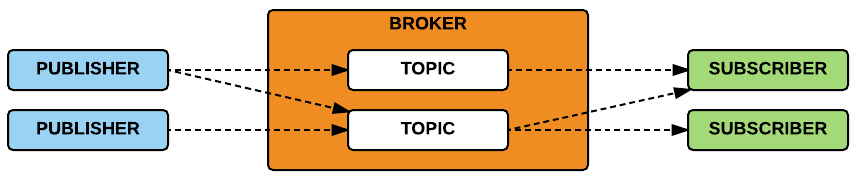
\includegraphics[width=\linewidth]{imagenes/sub-pattern-mqtt.png}
    \caption{Modelo publicación/suscripción \cite{disenio-mqtt}}
    \label{fig:figure13-mqtt-analysis}
\end{figure}

\subsection{Seguridad en MQTT}

La nota oficial de MQTT acerca de la seguridad de este (\textbf{mqtt.org}) \cite{mqtt}: \\

\textit{``Puedes pasar un nombre de usuario y una contraseña con un paquete MQTT en la V3.1 del protocolo. La encriptación a través de la red puede ser manejada con SSL, independientemente del protocolo MQTT en sí mismo (vale la pena señalar que SSL no es el más ligero de los protocolos, y añade una sobrecarga de red significativa). Se puede añadir seguridad adicional mediante una aplicación que cifre los datos que envía y recibe, pero esto no es algo integrado en el protocolo, con el fin de mantenerlo simple y ligero.``}\\

Aquí tenemos dos puntos a considerar:

\begin{enumerate}
    \item La autenticación es totalmente opcional
    \item Si se realiza la autenticación, el cifrado no se utiliza por defecto (las credenciales se envían en texto claro). Los ataques MITM aún pueden ser ejecutados para robar contraseñas.
\end{enumerate}

\subsection{Fases de un ataque}

Para poder contrarrestar un ataque debemos conocer las fases de este, por esto vamos a hacer un \textbf{test de intrusión} o \textbf{Pentest}. Esto es una prueba de seguridad ofensiva que simula un ataque real en un entorno controlado. El objetivo principal de este tipo de pruebas es identificar las posibles brechas en la seguridad de un sistema de manera que, al simular el comportamiento de los atacantes reales, podamos descubrir vulnerabilidades y agujeros de seguridad que necesiten ser corregidos para que no sean explotados por parte de atacantes reales. \cite{pentesting} \\

Las fases y tecnologías dentro de cada fase que nos encontramos son:

\begin{enumerate}
    \item \textbf{Reconocimiento}, se recolecta información del sistema de forma activa o pasiva. En este caso se van a usar herramientas como nmap o netstat para recopilar información de dominios, IPs, puertos y servicios.
    \item \textbf{Análisis de vulnerabilidades}, aquí se analizará la información recopilada de la fase de reconocimiento. Se puede investigar por internet posibles vulnerabilidad, por ello se puede mencionar a \textbf{CVE} \footnote{https://cve.report/vendor/mqtt}, para conocer posibles vulnerabilidad.
    \item \textbf{Explotación}, en esta fase se realizan las acciones necesarias para poder comprometer al sistema, los usuarios o la información que se maneja. Para este proyecto se usará \textbf{Metasploit}, es una herramienta que proporciona información acerca de vulnerabilidades de seguridad y ayuda en test de penetración.
\end{enumerate}

}

\input{capitulos/06_Diseño}

\chapter{Implementación}
{\color{blue}



La implementación de la aplicación se realiza con \textbf{Kaa IoT} tal y como se analizo anteriormente \ref{eleccion-framework}. Para empezar a usar el framework, hay que registrarse en sistema. Una vez registrados tendremos acceso a nuestro \textit{dashboard} \footnote{Hace referencia al cuadro de mandos al que tenemos acceso para interactuar con nuestro dispositivo y todas las posibles configuraciones}. En este capítulo se trata de mostrar una guía con la que se consiga conectar un dispositivo, recoger y enviar datos desde/hacia el dispositivo y mostrar las opciones que nos ofrece Kaa IoT como framework IoT. Para empezar, vamos a conectar nuestro primer dispositivo.

\begin{figure}[hb!]
    \centering
    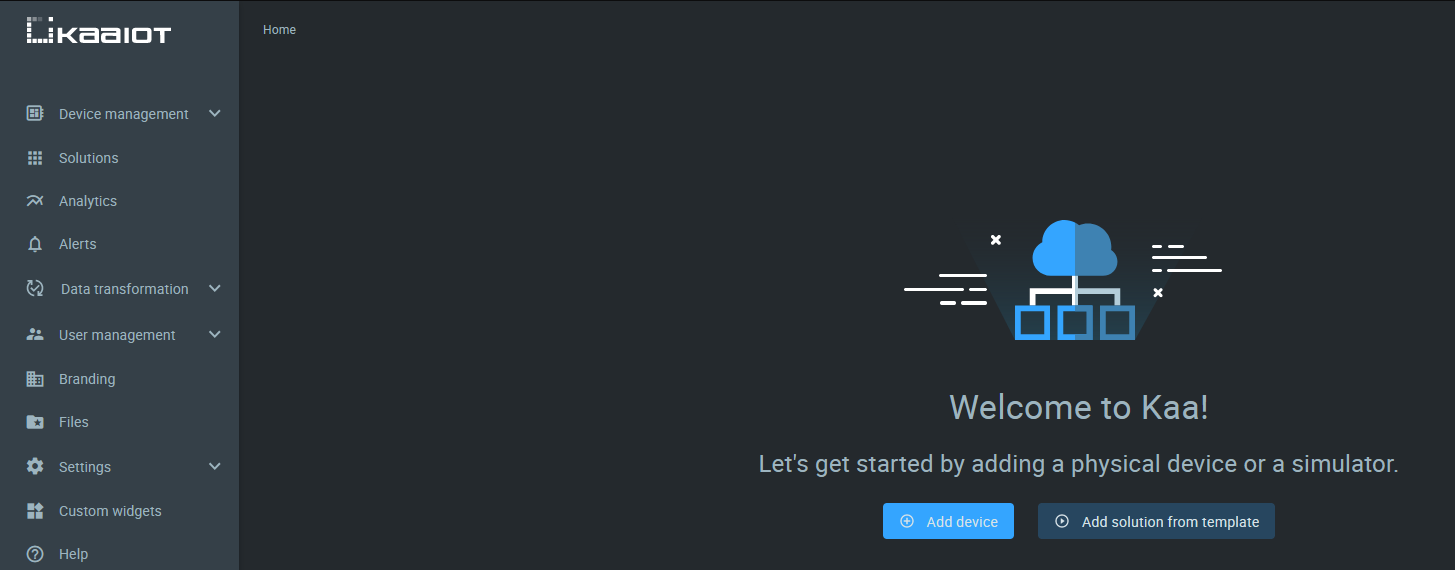
\includegraphics[width=\linewidth]{imagenes/dashboard.png}
    \caption{Dashboard Kaa IoT.}
    \label{fig:figure5}
\end{figure}


\section{Conectar dispositivo}

En este apartado se trata de explicar el proceso de conexión de un dispositivo con nuestra aplicación, desde crear un endpoint hasta ver la información del dispositivo en nuestra interfaz de usuario. Esto engloba varios términos y conceptos que se van a definir a continuación.

\subsection{Términos y conceptos} \label{initial-terms}

\subsubsection{Endpoints}

Los endpoints representan ``el elemento de las cosas`` del IoT. Un endpoint es cualquier dispositivo terminal que se quiera gestionar, en nuestro caso desde Kaa IoT. Un endpoint puede ser un dispositivo físico o una emulación de software del mismo. Todos los datos que llegan a la aplicación están asociados a endpoints. \cite{kaaiotConcepts}

Para ser precisos, un endpoint puede ser una unidad menor que un dispositivo, lo que significa que un dispositivo físico puede incluir múltiples endpoints. Por ejemplo, quieres gestionar un termostato, para que el aire acondicionado se encienda y apague automáticamente a cierta temperatura.

Se puede gestionar el termostato de una de las siguientes maneras:

\begin{itemize}
    \item Toda la unidad del termostato actúa como un endpoint único que intercambia datos con el servidor.
    \item Los componentes del termostato, como los sensores de temperatura y humedad, interruptor de encendido/apagado, actúan como endpoints individuales.
\end{itemize}

\subsubsection{ID de Endpoint}

El ID de endpoints se utiliza para identificar de forma única un endpoint dentro de una instancia. Un ID de endpoints suele ser un UUID generado automáticamente por el framework en el momento de crear un nuevo endpoint. No obstante, también se permiten los ID de endpoints definidos por el usuario. El ID de los endpoints no puede modificarse una vez creado.

Todos los datos de los endpoints, como los atributos de los metadatos, los puntos de datos de series temporales recopilados, los comandos, etc., están asociados a un ID de endpoint específico. Siempre que recupere o gestione datos relacionados con endpoints en Kaa, principalmente a través de la API REST, se verá los ID de endpoints.

\subsubsection{Token del Endpoint} \label{llamada-mqtt}

Los tokens de endpoints se utilizan para la identificación de endpoints cuando se intercambian datos relacionados con los endpoints, utilizando los protocolos compatibles basados en MQTT y HTTP. Los tokens de endpoint son únicos dentro de una aplicación IoT y se asignan exactamente a un endpoint.

Cuando llega un mensaje de un cliente, el token del endpoint se resuelve en el correspondiente ID del endpoint. Un ejemplo sobre el protocolo MQTT, el token del endpoint va dentro de la llamada MQTT, por ejemplo:

\begin{lstlisting}[language=HTML]
kp1/<APPLICATION_VERSION>/epmx/<ENDPOINT_TOKEN>/get
\end{lstlisting}

Normalmente, los tokens son cadenas generadas automáticamente por el framework, pero también se puede crear un token como el usuario quiera, por ejemplo, por el número de serie del dispositivo, dirección MAC, etc.

\subsubsection{Metadatos del endpoint}

Los metadatos de los endpoints son un conjunto de atributos clave-valor asociados a un endpoint. Se representan en el framework como un documento JSON de formato arbitrario.

Los metadatos de endpoints suelen incluir alguna información relacionada con los endpoints, como la ubicación, la descripción, el número de serie, la versión de hardware, etc. Los metadatos se almacenan en el servicio de registro de endpoints y pueden leerse o actualizarse de dos maneras:

\begin{itemize}
    \item A través de la capa de comunicación.
    \item A través de la API REST.
\end{itemize}

También se pueden gestionar los metadatos mediante la interfaz de usuario del framework.

\subsubsection{Aplicaciones y versiones}

Las aplicaciones en Kaa IoT sirven como contenedores para endpoints de diferentes tipos. Se puede tener una aplicación que contenga todos los endpoints que representan a un determinado dispositivo, y una aplicación para otro dispositivo, independiente de la otra aplicación. Las aplicaciones IoT también albergan toda la configuración del sistema necesaria para que el framework conozca las capacidades de sus dispositivos conectados y cómo trabajar con ellos.

Puede pasar que ya hemos configurado nuestro dispositivo, pero queremos implementar una nueva característica. Al implementarla se actualiza el firmware del dispositivo y se empieza a desplegar pero, ¿como diferenciamos entre los dispositivos que ya tienen el nuevo firmware y las que no? Aquí aparecen las versiones de una aplicación.

Cada aplicación puede tener varias versiones al mismo tiempo. Cada versión representa un conjunto de capacidades soportadas por los endpoints. En cualquier momento, cada endpoint está asociado a una versión de su aplicación. El conocimiento de la versión actual de la aplicación de un endpoint ayuda al framework a entender qué funcionalidad soporta el endpoint, cómo se formatean los datos, etc. Se puede utilizar las versiones para hacer evolucionar los dispositivos añadiendo o retirando funcionalidades mientras mantiene sus versiones antiguas en funcionamiento. Para diferenciar llamadas entre versiones se puede indicar como hemos visto en \ref{llamada-mqtt}.

\subsection{Pasos a seguir}

\subsubsection{Crear una aplicación y una versión}

Como hemos visto en \ref{initial-terms}, para registrar un endpoint en nuestro framework necesitamos una aplicación y una versión de esta. Esto podemos gestionarlo desde la interfaz de usuario, concretamente en la sección ``Applications``, una vez en la sección usaremos el botón de ``Add application``. Introduciremos el nombre de la aplicación (campo obligatorio) y tendremos la posibilidad de introducir una descripción. En nuestro caso la aplicación se llamará ``TFG-DASIoT``. \\

Hay que tener en cuenta que tanto las aplicaciones como las versiones tienen:

\begin{itemize}
    \item Nombres autoasignados e inmutables que suelen ser como  \textbf{7bfdd6b9-ff44-4098-a4dc-58c0f3c9f693-v1}. Se utilizarán para las llamadas a la API, la integración con el cliente, etc.
    \item Nombres de visualización arbitrarios que se pueden cambiar en cualquier momento. Estos nombres se utilizan en la interfaz de usuario de la plataforma para una mejor experiencia de usuario. Por ejemplo, en nuestro caso el nombre de la aplicación y la descripción que hayamos puesto.
\end{itemize}

\begin{figure}[hb!]
    \centering
    
\includegraphics[width=\linewidth]{imagenes/app-creada.png}
    \caption{Nombre y descripción de la aplicación}
    \label{fig:figure6}
\end{figure}

En la imagen también se puede observar como hay un identificador justo debajo del nombre que le hemos asignado a la aplicación, esto es para referenciar de manera univoca a esta. Y ahora que tenemos la aplicación, creamos una versión de esta.

\begin{figure}[ht!]
    \centering
    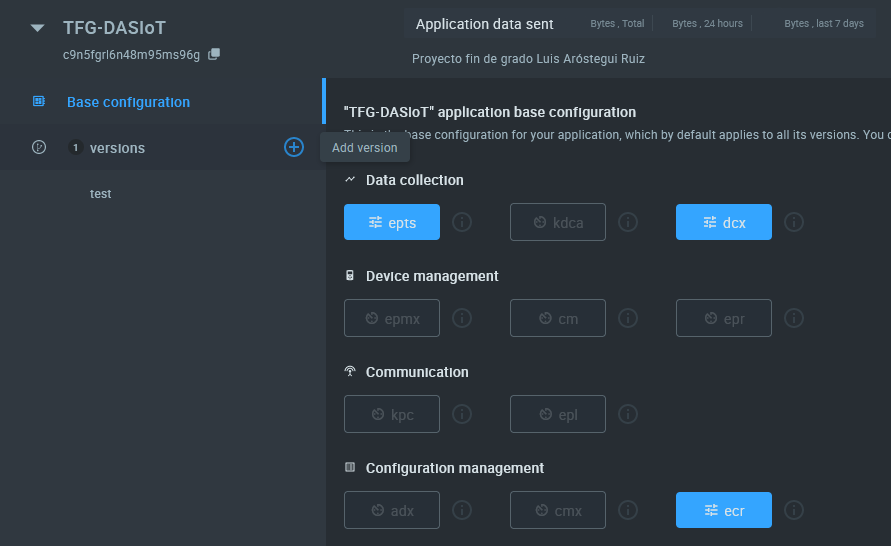
\includegraphics[width=\linewidth]{imagenes/app-version.png}
    \caption{Versiones de la aplicación}
    \label{fig:figure7}
\end{figure}

La primera versión que hemos creado se llama ``test``. Y en la información de la aplicación podemos ver los servicios que tenemos activos.

\begin{itemize}
    \item \textbf{Data collection}. \textit{epts}, se refiere al servicio de series temporales de endpoints. Recibe muestras de datos de endpoints y los transforma en series temporales. \textit{dcx}, es un servicio de recogida de datos, permite a los endpoints enviar muestras de datos de telemetría a la aplicación.
    \item \textbf{Configuration management}. \textit{ecr}, configuración del repositorio del endpoint, almacena los datos de configuración de los endpoints y proporciona una API REST para la gestión.
\end{itemize}

\subsubsection{Crear un endpoint}

En la sección de ``Devices`` de nuestro dashboard, podremos añadir un nuevo dispositivo. Aqui indicaremos, la aplicación a la que va a estar asociada el dispositivo, un nombre para nuestro endpoint y opcionalmente podremos añadir metadatos.

\begin{figure}[p]
    \centering
    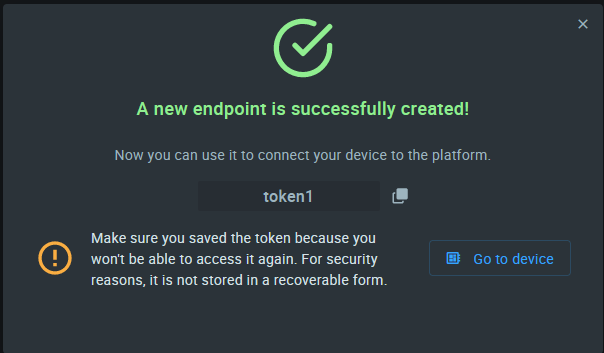
\includegraphics[width=\linewidth]{imagenes/device-added.png}
    \caption{Endpoint creado}
    \label{fig:figure8}
\end{figure}

\begin{figure}[p]
    \centering
    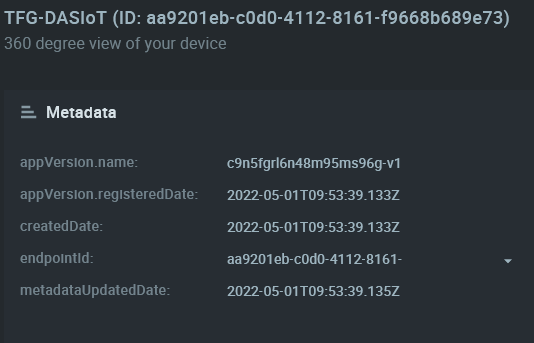
\includegraphics[width=\linewidth]{imagenes/device-created-view.png}
    \caption{Datos del dispositivo creado}
    \label{fig:figure9}
\end{figure}

En nuestro caso, para referirnos al endpoint lo hacemos mediante el \textit{token endpoint} \ref{llamada-mqtt}, que como vemos en \ref{fig:figure8}, se llama token1. Esto lo usaremos en nuestra llamada mqtt para hacer referencia a este dispositivo.\\

Para ver todos los datos del dispositivo se nos muestra como vemos en \ref{fig:figure9}. Donde podemos ver la aplicación a la que esta asociada, la fecha de creación y de su última actualización.

\newpage

\subsubsection{Conectar un cliente}

Una vez ya hemos creado nuestro primer endpoint, podemos conectar un cliente y obtener y enviar algunos metadatos. Como se analizó \ref{eleccion-framework}, Kaa IoT es un framework que soporta varios protocolos donde nos encontramos con HTTP y MQTT \ref{protocolos}.

Para hacer uso de los protocolos y completar la integración del cliente necesitaremos el nombre de la versión y el token del endpoint. En esta sección se va a mostrar como hacer uso de ambos protocolos, concretamente de las órdenes para poder ejecutar la conexión con nuestro dispositivo, en la sección de \textit{Pruebas} \ref{pruebas} se mostrarán los datos que obtenemos tras su ejecución.\\

\paragraph{Conexión mediante HTTP}

Para obtener todos los atributos de los metadatos con \textbf{HTTP} vamos a hacer uso de cURL \footnote{Es un proyecto de software consistente en una biblioteca y un intérprete de comandos orientado a la transferencia de archivos. Soporta los protocolos FTP, FTPS, HTTP, HTTPS, TFTP, SCP, SFTP, Telnet, DICT, FILE y LDAP, entre otros.} para enviar una solicitud de actualización de datos del dispositivo.

\begin{lstlisting}[language=bash]
curl - -location - -request POST 'https://connect.cloud.kaaiot.com:443/kp1/
<app-version-name>/epmx/<endpoint-token>/update/keys' \
- -data-raw '{
    "model": "BFG 9000",
    "mac": "00-14-22-01-23-45"
}'
\end{lstlisting}

Ejecutando esta instrucción añadiremos nuevos metadatos a nuestro dispositivo, concretamente la dirección física y el modelo de este.

\paragraph{Conexión mediante MQTT}

Para hacer la conexión mediante \textbf{MQTT} se ha optado por la opción de usar Python en su versión 3.10, obtenemos un código como el siguiente.

\begin{lstlisting}[language=Python]
import itertools
import json
import queue
import random
import string
import sys
import time

import paho.mqtt.client as mqtt
from decouple import config

KPC_HOST = config('KPC_HOST', cast=str)
KPC_PORT = config('KPC_PORT', cast=int)

APPLICATION_VERSION = config('APPLICATION_VERSION', cast=str)
ENDPOINT_TOKEN = config('ENDPOINT_TOKEN', cast=str)


class MetadataClient:

    def __init__(self, client):
        self.client = client
        self.metadata_by_request_id = {}
        self.global_request_id = itertools.count()
        get_metadata_subscribe_topic = f'kp1/{APPLICATION_VERSION}/epmx/{ENDPOINT_TOKEN}/get/#'
        self.client.message_callback_add(get_metadata_subscribe_topic, self.handle_metadata)

    def handle_metadata(self, client, userdata, message):
        request_id = int(message.topic.split('/')[-2])
        if message.topic.split('/')[-1] == 'status' and request_id in self.metadata_by_request_id:
            print(f'<--- Received metadata response on topic {message.topic}')
            metadata_queue = self.metadata_by_request_id[request_id]
            metadata_queue.put_nowait(message.payload)
        else:
            print(
                f'<--- Received bad metadata response on topic {message.topic}:\n{str(message.payload.decode("utf-8"))}')

    def get_metadata(self):
        request_id = next(self.global_request_id)
        get_metadata_publish_topic = f'kp1/{APPLICATION_VERSION}/epmx/{ENDPOINT_TOKEN}/get/{request_id}'

        metadata_queue = queue.Queue()
        self.metadata_by_request_id[request_id] = metadata_queue

        print(f'---> Requesting metadata by topic {get_metadata_publish_topic}')
        self.client.publish(topic=get_metadata_publish_topic, payload=json.dumps({}))
        try:
            metadata = metadata_queue.get(True, 5)
            del self.metadata_by_request_id[request_id]
            return str(metadata.decode("utf-8"))
        except queue.Empty:
            print('Timed out waiting for metadata response from server')
            sys.exit()

    def patch_metadata_unconfirmed(self, metadata):
        partial_metadata_udpate_publish_topic = f'kp1/{APPLICATION_VERSION}/epmx/{ENDPOINT_TOKEN}/update/keys'

        print(f'---> Reporting metadata on topic {partial_metadata_udpate_publish_topic}\nwith payload {metadata}')
        self.client.publish(topic=partial_metadata_udpate_publish_topic, payload=metadata)


def main():
    # Inicializar conexion con el servidor
    print(
        f'Connecting to Kaa server at {KPC_HOST}:{KPC_PORT} using application version {APPLICATION_VERSION} and endpoint token {ENDPOINT_TOKEN}')

    client_id = ''.join(random.choice(string.ascii_uppercase + string.digits) for _ in range(6))
    client = mqtt.Client(client_id=client_id)
    client.connect(KPC_HOST, KPC_PORT, 60)
    client.loop_start()

    metadata_client = MetadataClient(client)

    # Obtener los atributos de los metadatos del endpoint actual
    retrieved_metadata = metadata_client.get_metadata()
    print(f'Retrieved metadata from server: {retrieved_metadata}')

    # Actualizar parcialmente los metadatos del endpoint
    metadata_to_report = json.dumps({"model": "BFG 9001", "mac": "00-14-22-02-23-45"})
    metadata_client.patch_metadata_unconfirmed(metadata_to_report)

    time.sleep(5)
    client.disconnect()


if __name__ == '__main__':
    main()

\end{lstlisting}

La ejecución de este código produce el mismo efecto que el visto con HTTP. Se usa \textit{decouple} para evitar mostrar los datos de configuración de la aplicación, como el endpoint o la versión de la aplicación (lineas 12-16).
}

\section{Recogida de datos de un dispositivo}

\chapter{Pruebas} \label{pruebas}

Para realizar las pruebas, he tenido la oportunidad de usar una Raspberry PI \cite{raspberry-specs}. De esta manera he podido hacer uso de las funcionalidades de este dispositivo para mostrar de una manera más realista el potencial de la aplicación y también de explotar una vulnerabilidad.

\section{Conectar un cliente}

Tal y como vimos en \ref{connect-dispositivo}, una vez ya hemos creado nuestro primer endpoint, podemos conectar un cliente y obtener y enviar algunos metadatos. Como se analizó \ref{eleccion-framework}, Kaa IoT es un framework que soporta varios protocolos donde nos encontramos con HTTP y MQTT \ref{protocolos}. \\

Para hacer uso de los protocolos y completar la integración del cliente necesitaremos el nombre de la versión y el token del endpoint. En esta sección se va a mostrar como hacer uso de ambos protocolos, concretamente de las órdenes para poder ejecutar la conexión con nuestro dispositivo, en la sección de \textit{Pruebas} \ref{pruebas} se mostrarán los datos que obtenemos tras su ejecución.\\

\subsection{Conexión mediante HTTP} \label{http-connection}

Para obtener todos los atributos de los metadatos con \textbf{HTTP} vamos a hacer uso de cURL \footnote{Es un proyecto de software consistente en una biblioteca y un intérprete de comandos orientado a la transferencia de archivos. Soporta los protocolos FTP, FTPS, HTTP, HTTPS, TFTP, SCP, SFTP, Telnet, DICT, FILE y LDAP, entre otros.} para enviar una solicitud de actualización de datos del dispositivo.

\begin{lstlisting}[language=bash]
curl - -location - -request POST 'https://connect.cloud.kaaiot.com:443/kp1/
<app-version-name>/epmx/<endpoint-token>/update/keys' \
- -data-raw '{
    "model": "Raspberry PI",
    "mac": "00-14-22-01-23-45"
}'
\end{lstlisting}

Ejecutando esta instrucción añadiremos nuevos metadatos a nuestro dispositivo, concretamente la dirección física y el modelo de este.

\subsection{Conexión mediante MQTT} \label{mqtt-connection}

Para hacer la conexión mediante \textbf{MQTT} se ha optado por la opción de usar Python en su versión 3.10, obtenemos un código como el siguiente.

\begin{lstlisting}[language=Python]
import itertools
import json
import queue
import sys
from subprocess import Popen, PIPE


class MetadataClient:

    def __init__(self, client, app_version, endpoint_token):
        self.client = client
        self.app_version = app_version
        self.endpoint_token = endpoint_token
        self.metadata_by_request_id = {}
        self.global_request_id = itertools.count()
        get_metadata_subscribe_topic = f'kp1/{self.app_version}/epmx/{self.endpoint_token}/get/#'
        self.client.message_callback_add(get_metadata_subscribe_topic, self.handle_metadata)

    def handle_metadata(self, client, userdata, message):
        request_id = int(message.topic.split('/')[-2])
        if message.topic.split('/')[-1] == 'status' and request_id in self.metadata_by_request_id:
            print(f'<--- Received metadata response on topic {message.topic}')
            metadata_queue = self.metadata_by_request_id[request_id]
            metadata_queue.put_nowait(message.payload)
        else:
            print(
                f'<--- Received bad metadata response on topic {message.topic}:\n{str(message.payload.decode("utf-8"))}')

    def get_metadata(self):
        request_id = next(self.global_request_id)
        get_metadata_publish_topic = f'kp1/{self.app_version}/epmx/{self.endpoint_token}/get/{request_id}'

        metadata_queue = queue.Queue()
        self.metadata_by_request_id[request_id] = metadata_queue

        print(f'---> Requesting metadata by topic {get_metadata_publish_topic}')
        self.client.publish(topic=get_metadata_publish_topic, payload=json.dumps({}))
        try:
            metadata = metadata_queue.get(True, 5)
            del self.metadata_by_request_id[request_id]
            return str(metadata.decode("utf-8"))
        except queue.Empty:
            print('Timed out waiting for metadata response from server')
            sys.exit()

    def patch_metadata_unconfirmed(self, metadata):
        partial_metadata_update_publish_topic = f'kp1/{self.app_version}/epmx/{self.endpoint_token}/update/keys'

        print(f'---> Reporting metadata on topic {partial_metadata_update_publish_topic}\nwith payload {metadata}')
        self.client.publish(topic=partial_metadata_update_publish_topic, payload=metadata)

    def hardware_devices(self):
        return Popen(['lsusb'], stdout=PIPE, encoding='utf-8').communicate()[0]

    def set_metadata(self):
        metadata_to_report = json.dumps(
            {"model": "Raspberry PI",
             "mac": "b8-27-eb-f8-00-af",
             "devices": self.hardware_devices()
             }
        )
        return metadata_to_report

\end{lstlisting}

La ejecución de este código produce un efecto similar que el visto con HTTP. En este caso se ha creado una clase \textit{MetadataClient}, su objetivo es el de actualizar los metadatos del dispositivo en nuestra aplicación. Cada vez que se establece la conexión se analiza los dispositivos conectados a la Raspberry y se envían a la aplicación (como ejecutar en la terminal de linux, lusb).


\begin{figure}[p]
    \centering
    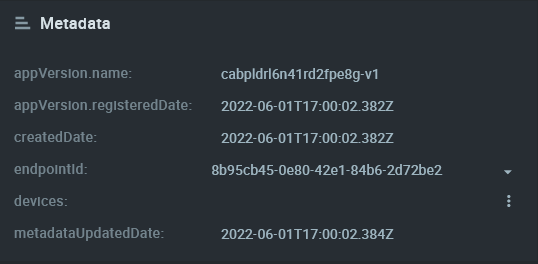
\includegraphics[width=\linewidth]{imagenes/metadata-old.png}
    \caption{Metadatos una vez creada nuestra aplicación}
    \label{fig:figure11}
\end{figure}


\section{Recogida de datos y ejecución de comandos de un dispositivo}


\subsection{Envio de datos mediante MQTT}

Al igual que en la sección \ref{mqtt-connection} tenemos un código para hacer el envió de datos y la ejecución de comandos, para ello definimos dos endpoints, uno para encender un led y el otro para apagar un led. \\


El código es el siguiente:

\begin{lstlisting}[language=Python]
import json
import signal
import time

from gpiozero import LED, CPUTemperature


def temp_data():
    cpu = CPUTemperature()
    return cpu.temperature


class KaaClient:

    def __init__(self, client, app_version, endpoint_token, host, port):
        self.client = client
        self.app_version = app_version
        self.endpoint_token = endpoint_token
        self.host = host
        self.port = port
        self.metadata_update_topic = f'kp1/{self.app_version}/epmx/{self.endpoint_token}/update/keys'
        self.data_collection_topic = f'kp1/{self.app_version}/dcx/{self.endpoint_token}/json'

        self.led = LED(17)

        command_turn_on_topic = f'kp1/{self.app_version}/cex/{self.endpoint_token}/command/turnon/status'
        self.client.message_callback_add(command_turn_on_topic, self.handle_turn_on_command)
        self.command_turn_on_result_topik = f'kp1/{self.app_version}/cex/{self.endpoint_token}/result/turnon'

        command_turn_off_topic = f'kp1/{self.app_version}/cex/{self.endpoint_token}/command/turnoff/status'
        self.client.message_callback_add(command_turn_off_topic, self.handle_turn_off_command)
        self.command_turn_off_result_topik = f'kp1/{self.app_version}/cex/{self.endpoint_token}/result/turnoff'

    def connect_to_server(self):
        print(
            f'Connecting to Kaa server at {self.host}:{self.port} using application version {self.app_version}'
            f' and endpoint token {self.endpoint_token}')
        self.client.connect(self.host, self.port, 60)
        print('Successfully connected')

    def disconnect_from_server(self):
        print(f'Disconnecting from Kaa server at {self.host}:{self.port}...')
        self.client.loop_stop()
        self.client.disconnect()
        print('Successfully disconnected')

    def compose_data_sample(self):
        return json.dumps([
            {
                "timestamp": int(round(time.time() * 1000)),
                "temperature": int(temp_data())
            }
        ])

    def on_message(client, userdata, message):
        print(f'<-- Received message on topic "{message.topic}":\n{str(message.payload.decode("utf-8"))}')

    def handle_turn_on_command(self, client, userdata, message):
        print(f'<--- Received "turn on" command on topic {message.topic} \nTurning on...')
        self.led.on()
        command_result = self.compose_command_result_payload(message)
        print(f'command result {command_result}')
        client.publish(topic=self.command_turn_on_result_topik, payload=command_result)

    def handle_turn_off_command(self, client, userdata, message):
        print(f'<--- Received "turn on" command on topic {message.topic} \nTurning off...')
        self.led.off()
        command_result = self.compose_command_result_payload(message)
        print(f'command result {command_result}')
        client.publish(topic=self.command_turn_on_result_topik, payload=command_result)

    def compose_command_result_payload(self, message):
        command_payload = json.loads(str(message.payload.decode("utf-8")))
        print(f'command payload: {command_payload}')
        command_result_list = []
        for command in command_payload:
            commandResult = {"id": command['id'], "statusCode": 200, "reasonPhrase": "OK", "payload": "Success"}
            command_result_list.append(commandResult)
        return json.dumps(
            command_result_list
        )


class SignalListener:
    keepRunning = True

    def __init__(self):
        signal.signal(signal.SIGINT, self.stop)
        signal.signal(signal.SIGTERM, self.stop)

    def stop(self, signum, frame):
        print('Shutting down...')
        self.keepRunning = False

\end{lstlisting}

Con este código se entra en un bucle donde se van haciendo llamadas al dispositivo y recogiendo información. La información que nos llega viene en formato JSON. Se usa la librería \textit{gpiozero} para encender/apagar el led y obtener la temperatura de la CPU. \\

También se ha creado un fichero para cargar la configuración necesaria (endpoint ID, host, puerto) y ejecutar el programa.

\begin{lstlisting}[language=Python]

import random
import string
import time

from metadataClient import MetadataClient
from kaaClient import KaaClient
from kaaClient import SignalListener

import paho.mqtt.client as mqtt
from decouple import config

KPC_HOST = config('KPC_HOST', cast=str)
KPC_PORT = config('KPC_PORT', cast=int)

APPLICATION_VERSION = config('APPLICATION_VERSION', cast=str)
ENDPOINT_TOKEN = config('ENDPOINT_TOKEN', cast=str)


def main():
    print(
        f'Connecting to Kaa server at {KPC_HOST}:{KPC_PORT} using application version {APPLICATION_VERSION}'
        f' and endpoint token {ENDPOINT_TOKEN}')

    client_id = ''.join(random.choice(string.ascii_uppercase + string.digits) for _ in range(6))
    client = mqtt.Client(client_id=client_id)
    client.connect(KPC_HOST, KPC_PORT, 60)
    client.loop_start()

    metadata_client = MetadataClient(client, APPLICATION_VERSION, ENDPOINT_TOKEN)

    retrieved_metadata = metadata_client.get_metadata()
    print(f'Retrieved metadata from server: {retrieved_metadata}')

    metadata_to_report = metadata_client.set_metadata()
    metadata_client.patch_metadata_unconfirmed(metadata_to_report)

    time.sleep(5)
    client.disconnect()

    client = mqtt.Client(client_id=''.join(random.choice(string.ascii_uppercase + string.digits) for _ in range(6)))

    data_collection_client = KaaClient(client, APPLICATION_VERSION, ENDPOINT_TOKEN, KPC_HOST, KPC_PORT)
    data_collection_client.connect_to_server()

    client.on_message = data_collection_client.on_message

    client.loop_start()

    listener = SignalListener()
    while listener.keepRunning:

        payload = data_collection_client.compose_data_sample()

        result = data_collection_client.client.publish(topic=data_collection_client.data_collection_topic,
                                                       payload=payload)
        if result.rc != 0:
            print('Server connection lost, attempting to reconnect')
            data_collection_client.connect_to_server()
        else:
            print(f'--> Sent message on topic "{data_collection_client.data_collection_topic}":\n{payload}')

        time.sleep(3)

    data_collection_client.disconnect_from_server()


if __name__ == '__main__':
    main()


\end{lstlisting}

Se usa \textit{decouple} para evitar mostrar los datos de configuración de la aplicación, usando un fichero \textit{.env}. \\

Se muestra a continuación pruebas de la ejecución del código.


\begin{figure}[p]
    \centering
    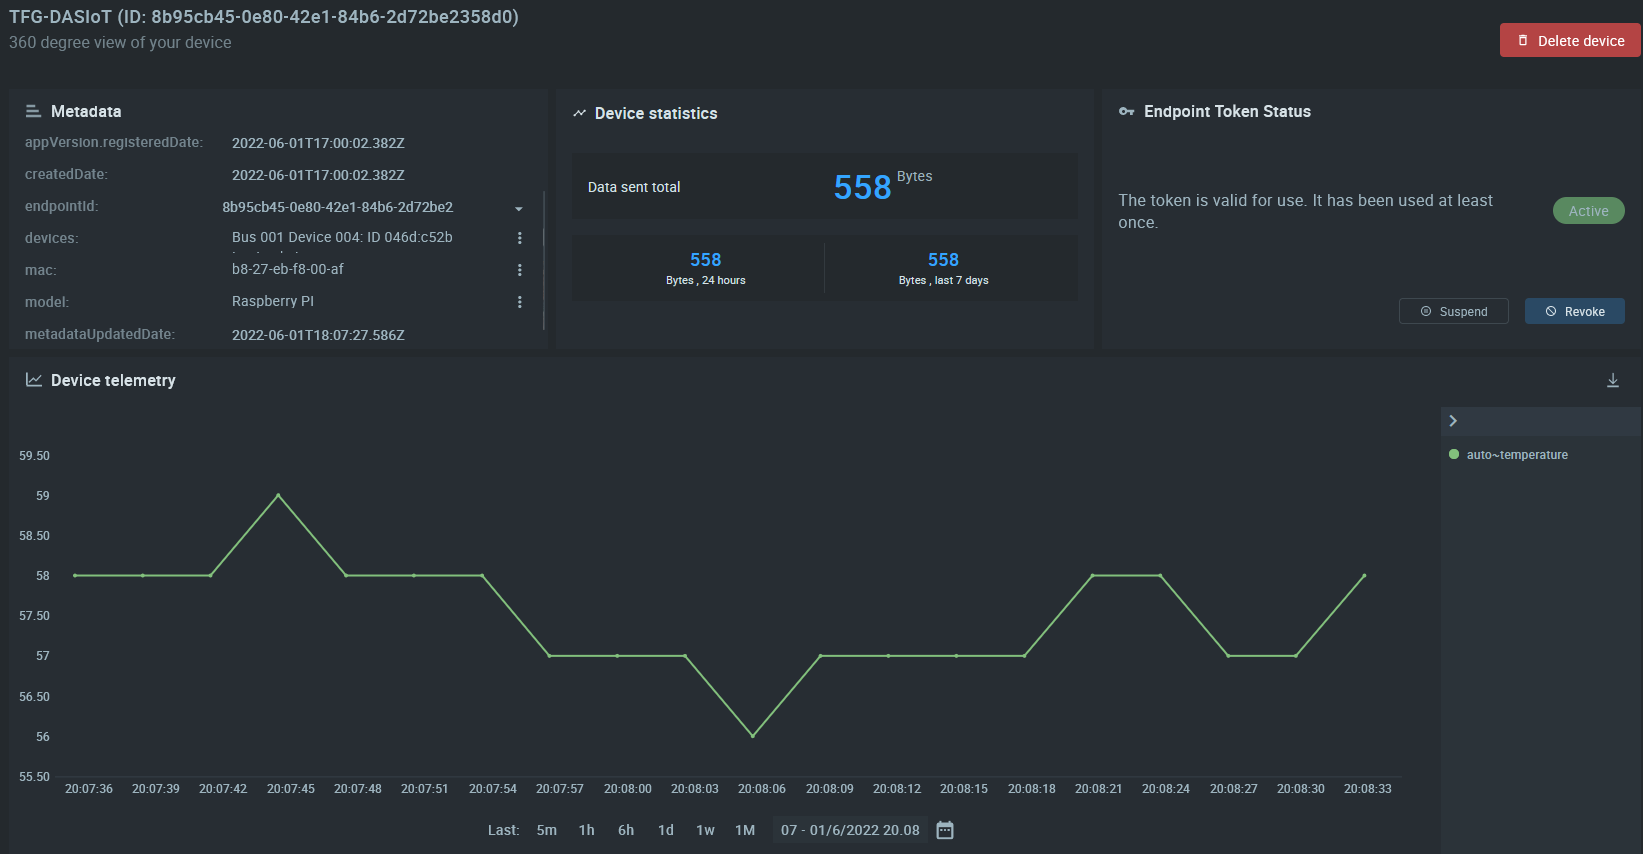
\includegraphics[width=\linewidth]{imagenes/data-execution.png}
    \caption{Metadatos actualizados y telemetría de la temperatura de la CPU}
    \label{fig:figure13}
\end{figure}

\begin{figure}[p]
    \centering
    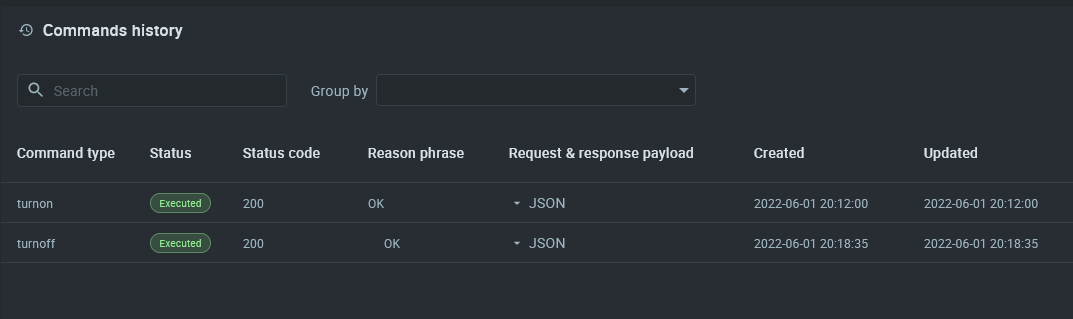
\includegraphics[width=\linewidth]{imagenes/command-execution.png}
    \caption{Encendido y apagado del led}
    \label{fig:figure14}
\end{figure}

\begin{figure}[p]
    \centering
    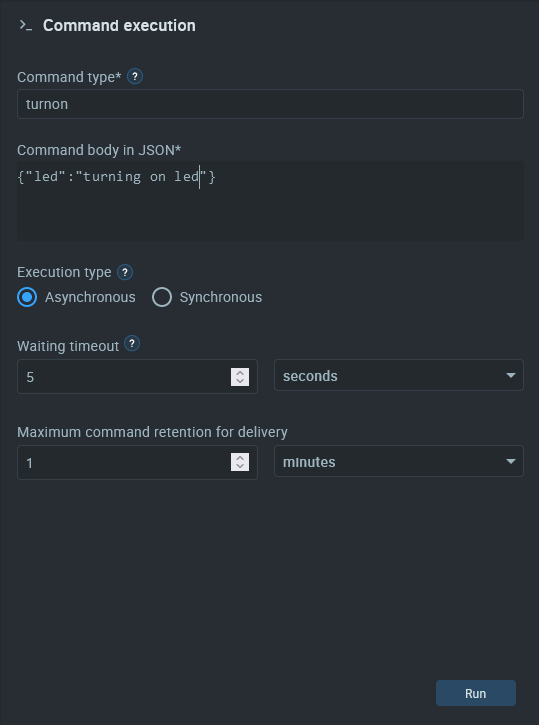
\includegraphics[width=\linewidth]{imagenes/turn-on-led.png}
    \caption{Petición de encendido del led}
    \label{fig:figure15}
\end{figure}

\begin{figure}[p]
    \centering
    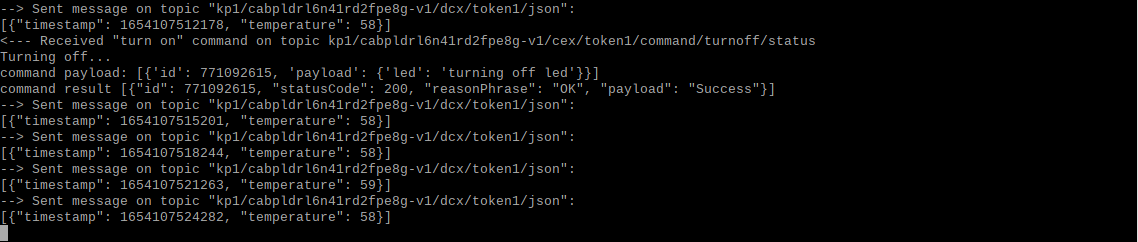
\includegraphics[width=\linewidth]{imagenes/2022-06-01-201846_1920x1080_scrot.png}
    \caption{Inicio de conexión y envio de datos a la aplicación}
    \label{fig:figure16}
\end{figure}

\begin{figure}[p]
    \centering
    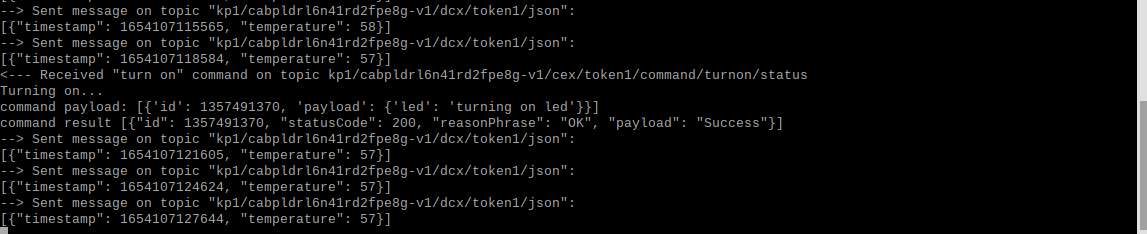
\includegraphics[width=\linewidth]{imagenes/2022-06-01-201209_1920x1080_scrot.png}
    \caption{Encendiendo el led}
    \label{fig:figure17}
\end{figure}

\begin{figure}[p]
    \centering
    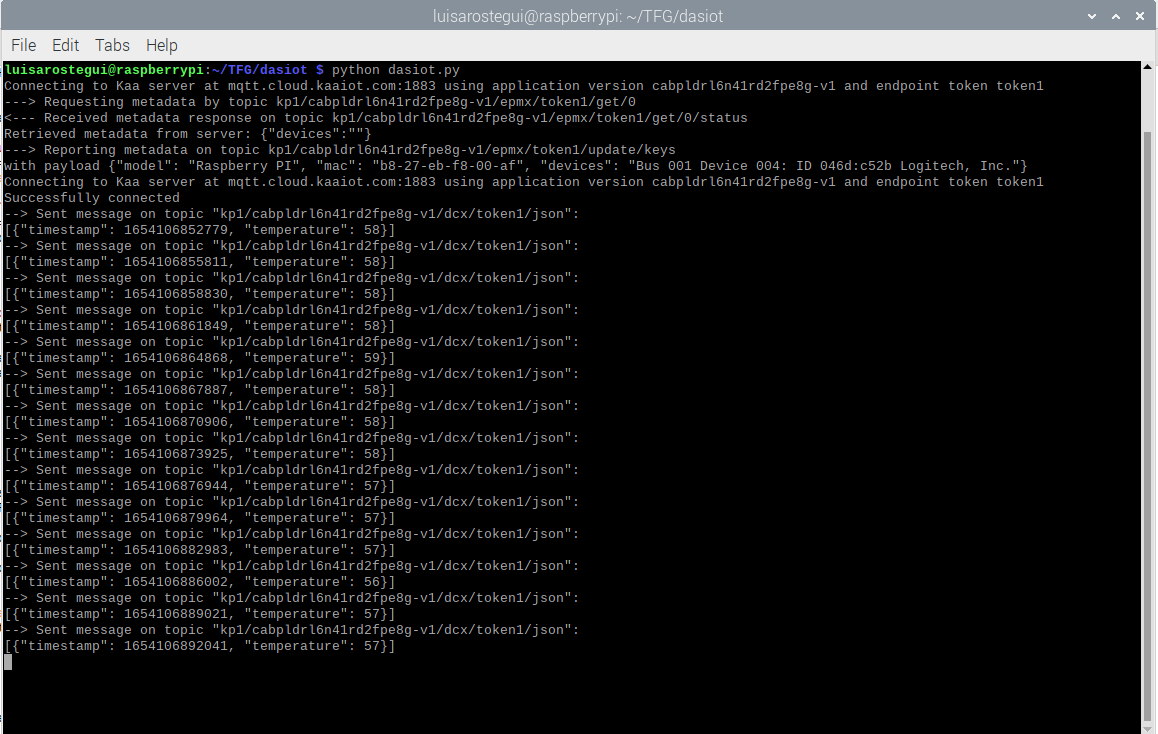
\includegraphics[width=\linewidth]{imagenes/2022-06-01-200813_1920x1080_scrot.png}
    \caption{Apagando el led}
    \label{fig:figure18}
\end{figure}

\newpage

\section{Escanear red}

Se muestra el escaneo de la red con \textbf{nmap}. \ref{fig:figure19-prueba}

\begin{figure}[p]
    \centering
    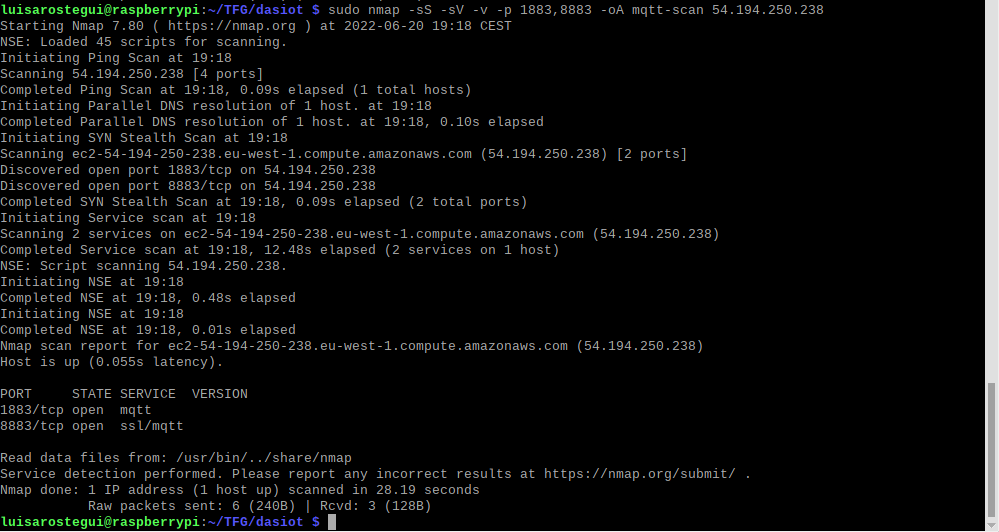
\includegraphics[width=\linewidth]{imagenes/2022-06-20-191838_1920x1080_scrot.png}
    \caption{Escaneo de red con nmap}
    \label{fig:figure19-prueba}
\end{figure}


\section{Explotación de una vulnerabilidad}

Se muestra el uso de Metasploit para iniciar sesión en la aplicación y poder enviar datos a la aplicación. \ref{fig:figure22-prueba} - \ref{fig:figure22.2-prueba} \\

\begin{figure}[p]
    \centering
    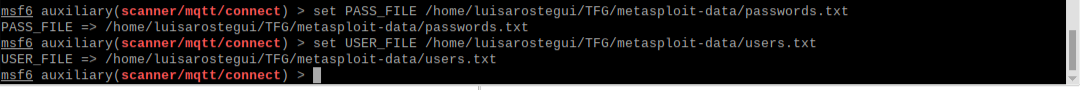
\includegraphics[width=\linewidth]{imagenes/2022-06-14-180947_1920x1080_scrot.png}
    \caption{Insertar PASS\_FILE y USER\_FILE}
    \label{fig:figure22-prueba}
\end{figure}

\begin{figure}[p]
    \centering
    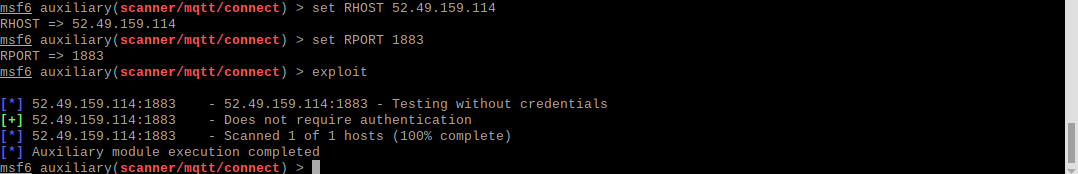
\includegraphics[width=\linewidth]{imagenes/2022-06-14-183011_1920x1080_scrot.png}
    \caption{Insertar host y puerto para ejecución. Resultado de la explotación}
    \label{fig:figure22.2-prueba}
\end{figure}

Para analizar la seguridad de crear un usuario para iniciar la conexión entre dispositivo y aplicación se ha escaneado el tráfico en el momento del inicio de sesión. \\

\begin{figure}[p]
    \centering
    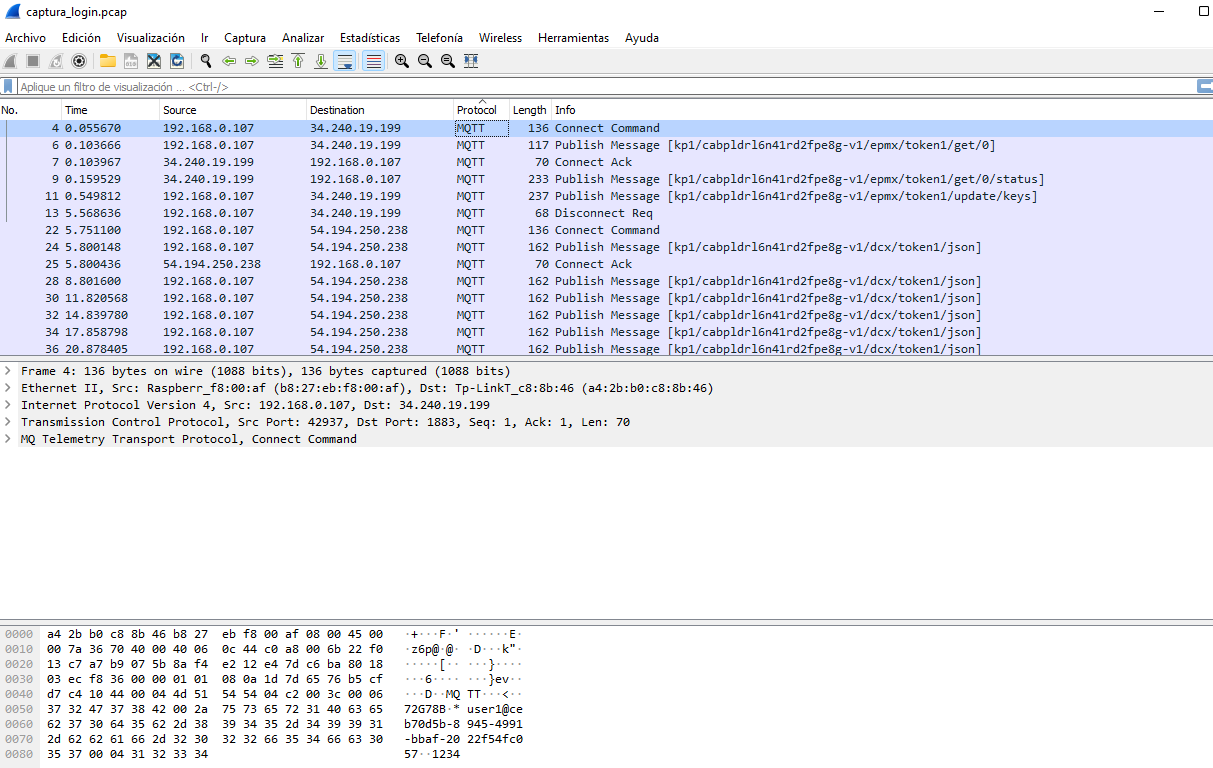
\includegraphics[width=\linewidth]{imagenes/Captura de pantalla 2022-06-26 190942.png}
    \caption{Captura de tráfico con tcpdump. Inicio de sesión}
    \label{fig:figure23-prueba}
\end{figure}

Si observamos los datos enviados al estar en el puerto 1883, todos los datos se envían sin encriptación y por tanto podemos leer las credenciales para el inicio de sesión. \ref{fig:figure23-prueba}

	% Análisis del problema
% 	\chapter{Análisis del problema}

	% Desarrollo
% 	\chapter{Diseño}
	
	% Implementación
% 	\chapter{Implementación}

 	% Pruebas
% 	\chapter{Pruebas}

	% Conclusiones
	\chapter{Conclusiones y trabajos futuros}

\section{Conclusiones}

Llegados a este punto del desarrollo del proyecto, se procede a comentar las conclusiones teniendo en cuenta cada objetivo especificado. \ref{sec:objetivos}

\begin{itemize}
    \item Para empezar se tenía que estudiar distintos frameworks para IoT y analizarlos. Debido a que se carecían de conocimientos relacionados con esta temática, se optó por la opción de empezar a estudiar los fundamentos y conocimientos existentes entorno a la temática elegida, tomando como referencia fuentes variadas, válidas y fiables. Este estudio permitió poder seleccionar un framework siguiendo unos requisitos que se ajustasen al proyecto para simplificar el desarrollo de los siguientes objetivos.
    \item En esta misma fase se estudiaron las distintas arquitecturas que existen dentro del IoT y las tecnologías asociadas a cada una de estas, punto clave para empezar a tener en cuenta posibles vulnerabilidades que se pueden explotar en la ultima fase del proyecto y de esta manera seleccionar un framework con que poder crear una aplicación basándonos en una posible vulnerabilidad de algunas de las tecnologías que podríamos llegar a usar.
    \item En la sección de análisis, concretamente para la búsqueda de un framework, también fue parte de estudio la diferencia entre middleware y framework. En varios artículos no hay una diferencia clara entre ambas, es un concepto algo ambiguo, que incluso aquí se puede añadir el concepto de plataforma. Por esto, se deja clara una sección de middleware y framework, y a que nos referimos cuando hablamos de cada una de ellas.
    \item De middleware y framework, podemos pasar a tecnologías y protocolos, otra sección a la que se le dedicó parte del estudio, estos conceptos también son algo ambiguos y de todos los libros y artículos consultados, no se especifica como referirnos a cada uno, por esto se indica en el proyecto a que nos referimos cuando hablamos de tecnologías. Estas ambigüedades nos llevan a darnos cuenta de que el paradigma IoT esta madurando y que hay secciones que se tienen que terminar de especificar y estandarizar.
    \item Respecto al segundo objetivo, se seleccionó un framework tomando como referencia una serie de requisitos. Tras el desarrollo de la aplicación con este framework se obtiene como conclusiones, que todo aquello relativo al IoT al ser un mundo que se esta dando a conocer y es reciente poco a poco los frameworks se están haciendo más potentes, eficientes y seguros pero como contra esto implica un mayor precio por su uso. Siguen existiendo framework que se pueden usar sin necesidad de realizar ningún pago pero estos están desapareciendo poco a poco porque las empresas ven una oportunidad de negocio única.
    \item Para el objetivo de explotación de una vulnerabilidad, en un principio se pensaba que podría ser el objetivo al que dedicar más tiempo, sin embargo, debido a que se escogió MQTT como tecnología a la que explotar no fue muy complicado encontrar vulnerabilidades en este. Es una tecnología muy potente para la transferencia de mensajes, sin embargo, carece de seguridad hoy día y le queda un largo proceso de mejoría en este apartado y más teniendo en cuenta la cantidad de herramientas que existen para explotar una vulnerabilidad y la cantidad de atancantes que hay en el mundo.
    \item Una parte que engloba a todos los objetivos, es la planificación, este punto siempre puede llegar a generar falsas expectativas con los plazos que fijan pero en este caso, con la metodología que se optó por usar, se ha podido seguir el proyecto de una manera bastante fiable, habiendo pocos días de diferencia entre la fecha inicialmente fijada y la fecha de finalización del objetivo. Usar tecnologías como las que se mencionaron han ayudado a medir el tiempo que se le dedicó a cada tarea sin extenderse en una u otra más de lo debido, distribuyendo de manera equitativa el tiempo en cada una de ellas.
\end{itemize}

\section{Vías futuras}

Conforme se ha ido avanzando con el trabajo se han encontrado varios conceptos algo ambiguos que han requerido de una especificación para hacer referencia a ellos. Por tanto, este trabajo se puede seguir ampliando y algunas de las ideas son las siguientes:

\begin{itemize}
    \item Uno de los puntos principales que requieren de un estudio más profundo es la parte de tecnologías y protocolos, como ya se ha mencionado, es un apartado que no está estandarizado y es confuso leer entre libros y artículos como se refieren en un lugar a MQTT como protocolo y en otro lugar como tecnología, por esto reorganizar la idea de estos conceptos sería ideal para un futuro.
    \item Algo similar pasa con el concepto de framework, middleware y plataforma, no esta estandarizado, definir de una manera clara cada uno de estos conceptos sería clave para el futuro desarrollo de nuevas aplicaciones.
    \item Respecto a la aplicación, se puede seguir desarrollando para mostrar estadísticas más detalladas, una mayor seguridad en esta. Pedir un certificado SSL para usar el puerto 8883 y tener una conexión cifrada y así tener un sistema de autenticación más robusto que el actual. También se puede desarrollar un sistema de gestión de alertas, si en un momento dado la temperatura de nuestro dispositivo supera X valor, se puede mandar un correo y ejecutar un comando para apagar el dispositivo.
    \item Para la parte de explotación de vulnerabilidades, aquí se puede seguir investigando más vulnerabilidades tanto de MQTT como a otro nivel, como puede ser el hardware o software. Se optó por explotar una vulnerabilidad conocida pero para un futuro uso de la aplicación el uso de varios usuarios y dispositivos se pueden encontrar otros problemas que vulneren la aplicación.
\end{itemize}


	
	\newpage
	\bibliography{bibliografia}
	\bibliographystyle{unsrt}
	
\end{document}